\documentclass[a4paper,11pt]{report}
\usepackage[T2A]{fontenc}
\usepackage[utf8]{inputenc}
\usepackage[main=english,russian]{babel}
\usepackage{graphicx}
\usepackage{csquotes}
\usepackage[ruled,vlined]{algorithm2e}
\setlength {\marginparwidth}{2cm}
\usepackage{todonotes}
\graphicspath{ {images/} }
\hfuzz 6pt
\usepackage{hyperref}
\usepackage{tabularx,lipsum,environ,amsmath,amssymb,framed}

\makeatletter
\newcounter{problemCounter}
\newcommand{\problemtitle}[1]{\gdef\@problemtitle{#1}}% Store problem title
\newcommand{\probleminput}[1]{\gdef\@probleminput{#1}}% Store problem input
\newcommand{\problemquestion}[1]{\gdef\@problemquestion{#1}}% Store problem question
\newcommand{\theProblemCounter}{\arabic{problemCounter}}
\NewEnviron{problem}[2]{
    \begin{framed}
  \problemtitle{}\probleminput{}\problemquestion{}% Default input is empty
  \BODY% Parse input
  \par\addvspace{.5\baselineskip}
  \noindent
  \begin{tabularx}{\textwidth}{@{\hspace{\parindent}} l X c}
    \multicolumn{2}{@{\hspace{\parindent}}l}{\@problemtitle} \\% Title
    \textbf{Input:} & \@probleminput \\% Input
    \textbf{Question:} & \@problemquestion% Question
  \end{tabularx}
  \par\addvspace{.5\baselineskip}
  \end{framed}
  \refstepcounter{problemCounter}%
  \label{#1}
  \noindent\textbf{Problem~\theProblemCounter}
}
\makeatother



\title{
	{Applications of Genetic Algorithms on theoretical fully-autonomous road systems} \\
	{\large University of Birmingham} \\ 
	{
\includegraphics[scale=0.3]{uobcrest.jpg}}
}
\author{Sam Barrett, \ID \\ sjb786@student.bham.ac.uk \\ Programme: \programme \\ Supervisor: \supervisor \\ Word count: \input{|./wordcount.sh}}
\newcommand{\ID}{1803086}
\newcommand{\supervisor}{Miriam Backens}
\newcommand{\programme}{MSci Computer Science}



\begin{document}
\maketitle
\listoftodos
\tableofcontents
\chapter*{Abstract}\label{chap:Abs}
\begin{abstract}
  Efficiently routing vehicle traffic is fast becoming a key area of research. With the number of vehicles on the road increasing, existing infrastructure is under growing strain. Extending road networks is a costly process and requires ongoing, expensive maintenance.

  Human drivers do not make efficient use of the existing road network, and so many approaches are being investigated for increasing this efficiency, thereby increasing throughput on the same series of roads.

  In this paper I investigate the potential applications of Genetic Algorithms in this space. Building and evaluating a parallel cooperative coevolutionary algorithm (PCCGA), utilising Bézier curves to encode individuals in each sub-population.

  I conclude that this approach has the potential, given more research and development time, to consistently produce feasible, safe routes for multiple agents across a network of roads.


\end{abstract}
%%% Local Variables:
%%% mode: latex
%%% TeX-master: "report"
%%% End:

\chapter{Introduction}\label{chap:Intro}


\chapter{Background}\label{chap:Background}
\section{Genetic Algorithms}

\subsection{History}\todo{Decide whether to keep this section}

Genetic algorithms (GAs) are a type of meta-heuristic optimisation technique that employ the same rationale as classical evolution seen in nature.

Genetic Algorithms can trace their origins back to the late 1960s when they were first proposed by John Holland, though he then referred to them as \textit{Genetic Plans}\footnote{This distinction was made to emphasise the \textit{``centrality of computation in defining and implementing the plans''}~\cite{hollandAdaptationNaturalArtificial1992}}. Holland went on to write the first book on the subject titled \textit{Adaptation in Natural and Artificial Systems}\cite{hollandAdaptationNaturalArtificial1992} in 1975. The field did not find much reception with Holland stating in the preface to the 1992 rerun:

\begin{displayquote}
\textit{``When this book was originally published I was very optimistic, envisioning extensive reviews and a kind of `best seller' in the realm of monographs. Alas! That did not happen.''}
\end{displayquote}

However, in the early nineties, Genetic algorithms surged in popularity along with the area of Artificially Intelligent planning as a whole, leading to Holland republishing his book and solidifying his position as the field's founder.

\subsection{Definition}
In a general sense, optimisation techniques work to find the set of parameters $\mathcal{P}$ that minimise an objective function $\mathcal{F}$. 
Genetic algorithms approach this by representing these sets as individuals in a population, $P$. Over the course of multiple generations, the best solutions are determined and promoted until termination criteria are met or the maximum number of generations is reached.

As our candidates are essentially a collection of parameters to the function we are trying to optimise, we can extend our metaphor further by mapping each element of a individual to a \textit{gene} in a individual's genome. 

The representation we use in a GA is problem specific. Often we have to provide functions to facilitate the mapping between the problem specific set of possible solutions and the encoded genotype space in which we optimise. The most basic representation being a string of binary numbers.

An individual's characteristics and genetic information is normally encapsulated within the Phenotype. Here not only the genetic information of the Genotype but also additional information, such as fitness, is stored in order to prevent it from being re-calculated as often.

In general, an individual's phenotype is the real-world representation of the candidate solution. The genotype is the low-level representation on which the genetic operators can operate. I will generally refer to both as an individual throughout this paper as the distinction is only necessary at the implementation level.

Genetic algorithms are both \textit{probabilistically optimal} and \textit{probabilistically complete}\cite{kalaOnroadIntelligentVehicles2016} meaning that: given infinite time, not only will the algorithm find \textit{a} solution, (if one exists), it will find \textbf{the} optimal solution from the set of all possible solutions, $\mathcal{P}^*$.

\begin{algorithm}[H]
	\label{alg:GenericGA}
	\SetAlgoLined
	\KwResult{Best Solution, $p_{ \texttt{best}}$}	
	Generate initial population, $P_0$ of size $n$\;
	Evaluate fitness of each individual in $P_0$, $\{F(p_{0,1},\ldots, p_{0,n})\}$\;
	\While{termination criteria are not met}{
		\textbf{Selection}: Select individuals from $P_t$ based on their fitness\;
		\textbf{Variation}: Apply variation operators to parents from $P_t$ to produce offspring\;
		\textbf{Evaluation}: Evaluate the fitness of the newly bred individuals\;
		\textbf{Reproduction}: Generate a new population $P_{t+1}$ using individuals from $P_t$ as well as the newly bred candidates.\;
		$t$++
	}
	return $p_{\texttt{best}}$

	\caption{Modern Generic Genetic Algorithm}
\end{algorithm}

\begin{figure}[htpb]
    \centering
    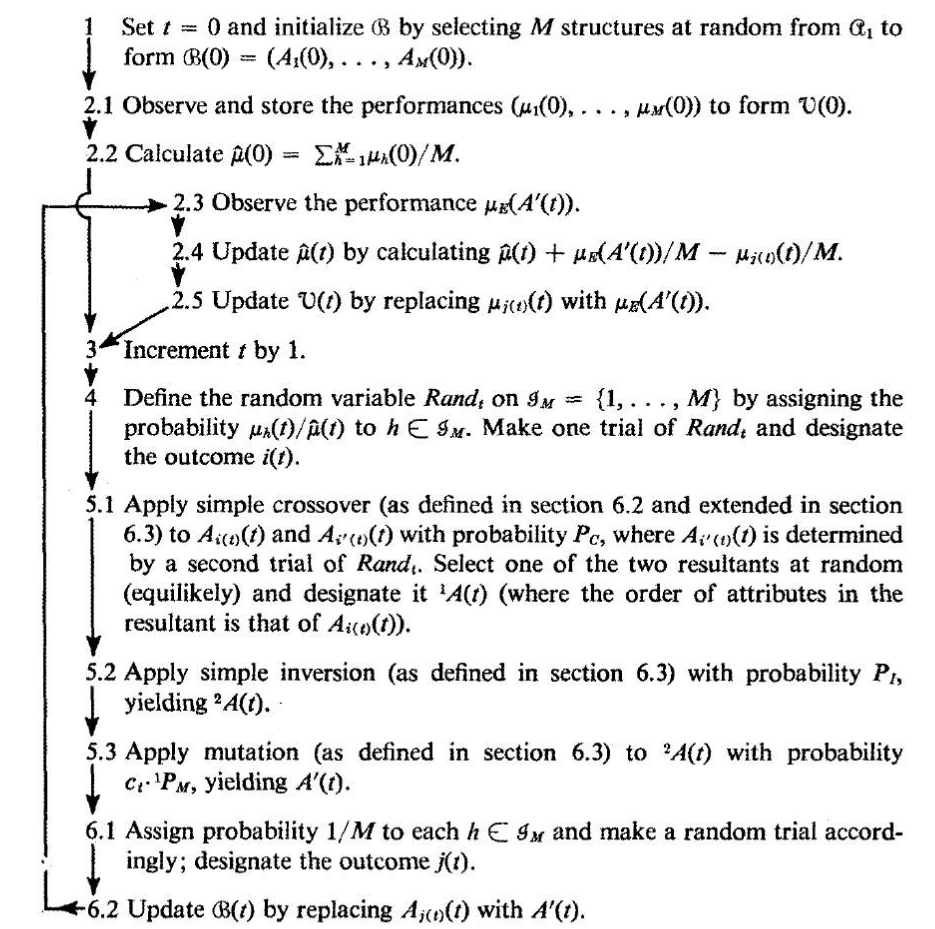
\includegraphics[width=\linewidth]{hollandAlg}
    \caption{GA outlined in Holland's Original Book\cite{hollandAdaptationNaturalArtificial1992}}
    \label{fig:hollandAlg}
\end{figure}

As you can see from Figure \ref{fig:hollandAlg} and Algorithm \ref{alg:GenericGA} the overall shape of GAs has not changed substantially over the course of the past 50 years. Being comprised of a series of operations that a starting population is piped through until criteria are met.

\subsection{Genetic Operators}\todo{Expand definitions of operators used in implementation section}
\label{subsec:GAOps}
In the following section I will outline the various genetic operations that take place in a GA, they can be seen in Algorithm~\ref{alg:GenericGA}. Any operators used and analysed in Chapter~\ref{chap:ClassicalApproach} will have more detailed explanations of their process.

\subsubsection{Selection}

The selection procedure is the process by which the next generation of individuals is created from the current population. Individuals are selected relative to their fitness as determined by the Objective (fitness) function $\mathcal{F}$. 

Some methods select only the best solutions by fitness. Others employ a more stochastic approach, such as roulette wheel selection, to increase diversity and reduce complexity.

\paragraph{Fitness Proportional Selection}\label{imp:FitPropSel}

Fitness proportional or Roulette wheel selection is a popular selection operator. It uses fitness to assign selection probability to each individual in a population.

The probability of selection for an individual $i$ with fitness $\mathcal{F}(i)$ can be expressed mathematically as:

\begin{equation}
    p_i = \frac{\mathcal{F}(i)}{ \sum^{N}_{j=1} \mathcal{F}(j)} 
\end{equation}

Where $N$ is the size of the population $P$

This is a simple approach but performs well and has very little performance overhead.

\paragraph{Ranked Selection}\label{imp:RankSel}

Ranked selection is an alternative selection method, it works on the assumption that the individuals in your population are closely grouped in fitness. The main difference of this method when compared to fitness proportional selection is that it ranks individuals based on relative fitness rather than absolute fitness.

The procedure can be written mathematically as:

Given a population $P$ of size $n$ ordered by fitness. We select the top \(\gamma\)-ranked individual, $x_{\gamma}$ with a probability $p(\gamma)$. Where \(\gamma\) is the rank and $p(\gamma)$ is the ranking function.

The ranking function can take different forms including both linear and exponential ranking.\todo[inline]{extend list to include all functions used}

Linear ranking is defined as:

\begin{equation}
p(\gamma)= \frac{\alpha + (\beta-\alpha) \cdot \frac{\gamma}{n-1}}{n}
\end{equation}

Where:

\begin{itemize}
  \item $\sum_{\gamma=0}^n p(\gamma) = 1$
  \item $\alpha + \beta = 2$
  \item $1 \leq \beta \leq 2$
\end{itemize}

\subsubsection{Variation}

Variation in a GA is the process of altering the genome individuals to further explore the search space via stochastic local search.
We perform this using two distinct sub-operations: Mutation and Crossover.
Here we can view crossover as the \textit{breeding} process and mutation as resembling the natural tendency for DNA to mutate over the course of generations.

\paragraph{Mutation}
In mutation we alter each gene with a set probability $p_m$ known as the \textit{mutation rate}. A standard value for a mutation rate is $ \frac{1}{L} $ but it can fall anywhere in the range $p_m \in [ \frac{1}{L} , \frac{1}{2} ] $ where $L$ is the length of the genome.

A low value for $p_m$ a new individual which can be shown to be \textit{close} to it's parents in the search space relative to their \textit{Hamming distance}\footnote{Hamming Distance: A metric for comparing two binary data strings. The Hamming distance between two strings is the number of bit position in which they differ.} if using a Binary coded GA. In real-coded GAs they can be shown to be close by the Euclidean distance between them.

In binary coded GAs we alter a given gene by \textit{flipping} it's value.
In real-coded GAs mutation operators include: 
\begin{itemize}
    \item Uniform Mutation
    \item Non-Uniform Mutation
    \item Gaussian Mutation 
\end{itemize}
\subparagraph{Uniform Mutation}
In uniform mutation, we select a parent $p$ at random and replace a randomly selected gene $c_i \in p$ with a uniformly random number $c_i' \in [u_i,v_i]$  where $u_i$ and $v_i$ are set bounds.

\paragraph{Gaussian Mutation}

In Gaussian mutation, we select a parent $p$ at random and randomly select a gene $c_{i} \in p$. We replace $c_{i}$ with a new value $c_{i}'$ which is calculated as follows:

\begin{equation}
  c_{i}' = \min(\max(\mathcal{N}(c_{i},\sigma_{i}), u_{i}), v_{i})
\end{equation}

Where $\mathcal{N}(c_{i},\sigma_{i})$ is a Gaussian distribution with a standard deviation \(\sigma_{i}\) and a mean of $c_{i}$. \(\sigma_{i}\) may depend on the length of the interval bound, $l_{i} = v_{i} - u_{i}$, typically (and in my implementation) $\sigma_{i} = \frac{1}{10}l_{i}$


\subsubsection{Crossover}

Crossover is a binary operation, taking two randomly selected \textit{parents} from the population $P_t$ with a probability $p_c \in [0,1]$ 

There are two major forms of crossover for binary coded GAs: $n>1$ point crossover and Uniform crossover. 

For real-coded GAs you instead have a selection of Crossover operators including:

\begin{itemize}
    \item Flat crossover
    \item Simple crossover
    \item Whole arithmetic crossover
    \item Local arithmetic crossover
    \item Single arithmetic crossover
    \item BLX-$\alpha$ crossover
\end{itemize}


\subparagraph{Simple (one point) Crossover}\label{imp:SimpCross}

For simple crossover, randomly select a crossover point, $i \in \{1,\ldots,n \}$. All values before this point are swapped between the two parents. For 2 parents, $p_1 = \left\{ x_1^{[1]},\ldots,x_n^{[1]}\right\}$ and $p_2 = \left\{ x_1^{[2]},\ldots,x_n^{[2]}\right\}$ this can be represented as:

\begin{equation}
    p_1' = \left\{ x_1^{[1]},x_2^{[1]}, \ldots, x_i^{[1]}, x_{i+1}^{[2]},\ldots, x_n^{[2]} \right\} 
\end{equation}

\begin{equation}
    p_2' = \left\{ x_1^{[2]},x_2^{[2]}, \ldots, x_i^{[2]}, x_{i+1}^{[1]},\ldots, x_n^{[1]} \right\}
\end{equation}

\subsubsection{Evaluation}
After developing potential new individuals, the fitness of these new individuals is calculated using the objective function, $\mathcal{F}$

\subsubsection{Reproduction}
Here the next generation of individuals is constructed. There are multiple potential methods employed here with the simplest being to just replace the lest fit individuals with additional copies of the fitter individuals, be they pre-existing or newly generated.

In this stage various heuristics or alternative strategies can be implemented to speed up or slow down the convergence rate. Whilst their fitness may be low, having a diverse population allows for more of the search space to be explored. If the algorithm converges too quickly it may get \textit{stuck} in local minima. 


\section{Bézier Curves}
\label{sec:back-bezier-curves}

In my implementation, I utilise Bézier curves to encode complex route arcs between a series of points. Here I will briefly outline their construction and mathematical basis.

Bézier curves were popularised by and named after French auto-body\footnote{so I feel it is quite fitting that they find use in $21^{st}$ century automotive problems} designer Pierre Bézier in the 1960s and are commonly found in computer graphics today. They are parametric curves made up of a series of \textit{control points} which contort the shape of a line to produce a curve of nearly any shape. Although their mathematical basis was established in 1912 by Sergei Bernstein in the form of Bernstein polynomials\cite{bernstein1912best}.

A Bézier curve is said to have a degree of $n-1$ where $n$ is the number of control points including the start and end point of the curve.

\subsection{Formal Definition}

Bézier curves can be simply explicitly defined for degrees of 1 through 4, however, the general case of $n$ points is more useful to us. In their general form they can be defined recursively or explicitly. I implement the recursive version as it is much more readable for a programming language that supports recursion.

They are defined recursively as follows:

\begin{equation}
    \textbf{B}_{P_0}(t) = P_0
\end{equation}

\begin{equation}
    \textbf{B}_{P_0,P_1,\ldots,P_n}(t) = (1-t)\textbf{B}_{P_0,P_1,\ldots,P_{n-1}}(t) + t\textbf{B}_{P_1,P_2,\ldots,P_n}(t)
  \end{equation}

  Where the initial curve $B = B_{P_{0},P_{1},\ldots,P_{n}}$ and the parameter $t$ is a real number in the range of $[0,1]$. Therefore, the smoothness of the curve is determined by the granularity of the parameter when realising the curve.

An example of how the parameter $t$ corresponds to points on the curve can be seen in Figure~\ref{fig:bezexample}, the red numbers indicate the value for $t$ that corresponds to the green points on the curve and the purple points correspond to the control points. I.e. $B(0.37)$ produces the coordinates for the first labelled point seen, where the curve shown is $B$.

\begin{figure}[ht]
  \centering
  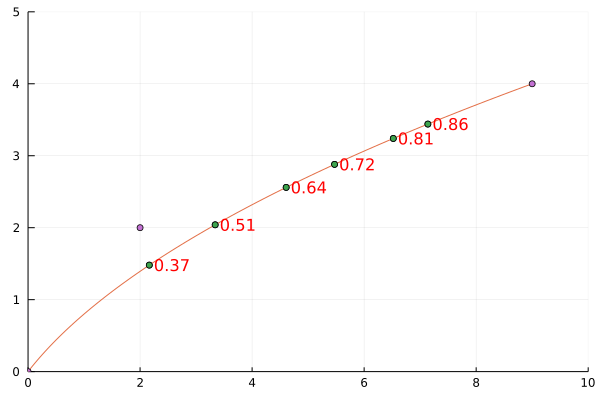
\includegraphics[scale=0.35]{figures/bezExample.png}
  \caption{\label{fig:bezexample} Example of a Bézier  curve with a random sample of points}
\end{figure}


\subsection{Length of a Bézier curve}
\label{subsec:back-bez-length}

The length of a Bézier curve is a non-trivial calculation and is best approximated as:

\begin{equation}
    L = \frac{(2L_c + (n-1)L_p)}{n+1}
\end{equation}

Where $L_c$ is chord length and $L_p$ is polygon length. This was proven by Jens Gravesen\cite{gravesenAdaptiveSubdivisionLength1997} in 1997.

Chord length is given by:

\begin{equation}\label{eq:bezlength}
  L_{c} = \sqrt{\left(P_{0_{x}} - P_{n_{x}}\right)^{2} + \left(P_{0_{y}} - P_{n_{y}}\right)^{2}}
\end{equation}
% √((first.x - last.x)^2 + (first.y - last.y)^2)

and polygon length by:

\begin{equation}
  L_{p} = \sum_{i=0}^{n-1} \sqrt{\left(P_{i_{x}} - P_{i+1_{x}}\right)^{2} + \left(P_{i_{y}} - P_{i_{y}}\right)^{2}}
\end{equation}

Or, alternatively:

\begin{equation}
  L_{p} = \sum_{i=0}^{n-1} L_{c}(B_{P_{i},P_{i+1}})
\end{equation}

\subsection{Subdivision of $n$-degree Bézier curves}
\label{sec:decasteljau}

Subdivision of Bézier curves is a key stage in the process of finding any intersections between two Bézier curves. The process of subdivision is performed using De Casteljau's algorithm. This algorithm was developed by Paul de Casteljau while working at Citroen in 1959 to work with the family of curves that would later be formalised into Bézier curves by Pierre Bézier\footnote{Bézier curves have also been called de Casteljau curves as much of his work preceded that of Pierre Bézier's}.

It is a simple procedure, given a Bézier curve $B$, it can be split at any arbitrary point $t \in [0,1]$ into two curves with control points of the form:

\begin{align}
  \beta_{1} &= B_{P_{0}}(t), B_{P_{0},P_1}(t), \ldots, B_{P_{0},\ldots,P_{n}}(t) \\
  \beta_{2} &= B_{P_{n}}(1-t), B_{P_{n},P_{n-1}}(1-t), \ldots, B_{P_{n},\ldots,P_{0}}(1-t)
\end{align}
\feedback{Should I change this superscript notation? subscript is being used to denote which control points are being considered.}

% \beta_1 = [ B[1:i](t) for i in 1:length(B) ]
% \beta_2 = [ B[i:length(B)](1-t) for i in length(B):-1:1 ]

\section{Fully Autonomous Road Networks}

Fully autonomous road networks are by no means a novel concept. They have appeared in fiction since the mid 20th century and have been a real possibility for the past decade. In a fully autonomous road networks \textit{(FARN)}s, all vehicles are self-operating with their routing either being determined on a vehicle-by-vehicle \textit{selfish} basis or by a larger system managing routes for all nearby agents. 

In the latter system protocols that promote the net increase in efficiency can be implemented. However, this sort of system will require a form of government mandate as a universal routing protocol would need to be established and implemented by all auto manufacturers; this is no small undertaking.

\section{Miscellaneous}

\subsection{Bounded Boxes}
\label{subsec:back_boundedboxes}

  A bounded box of a curve is defined as the box constructed from the points $(x_{min},y_{min}), (x_{min},y_{max}), (x_{max},y_{min}), (x_{max},y_{max})$ Where $x_{min,max}$ and $y_{min,max}$ are the minimum and maximum $x$ and $y$ values from all control points respectively. An example can be seen in Figure~\ref{fig:bboxeg}

 \begin{figure}[ht]
   \centering
   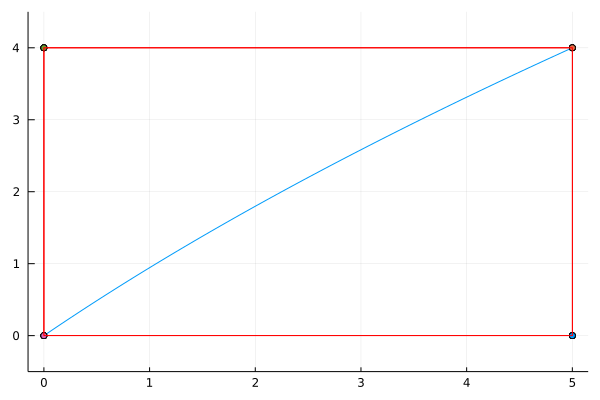
\includegraphics[scale=0.5]{figures/bbox_eg.png}
   \caption{\label{fig:bboxeg} A bounding box for a Bézier curve of degree 2}
 \end{figure}


%TC:macro \todo 1

%%% Local Variables:
%%% mode: latex
%%% TeX-master: "report"
%%% End:

\chapter{Literature Review}\label{chap:LitRev}


\section{Genetic algorithms for route generation}


Classical Genetic algorithms have seen research and applications in a number of fields over the past 40 years ranging from Heart disease diagnosis\cite{reddyHybridGeneticAlgorithm2020} to predicting the strength of concrete under various conditions\cite{shariatiPredictionConcreteStrength2020}.

There is a substantial and growing body of research specifically looking at the applications of GAs in route planning for autonomous agents, however, many are focusing on either abstract robotic agent planning in discrete search spaces or failing to take into account the wider environment of multiple agents.

\subsection{Genetic algorithms for cooperative route generation}

\paragraph{Cai \& Peng - Cooperative Coevolutionary Adaptive Genetic Algorithm in Path Planning of Cooperative Multi-Mobile Robot Systems\cite{caiCooperativeCoevolutionaryAdaptive2002}}

In this 2001 paper, Cai \& Peng give an example of a Cooperative Coevolutionary Adaptive Genetic Algorithm (CCAGA) for planning routes for multiple autonomous agents.

Their approach features a discrete grid-based search space featuring rectangular obstacles which the routes must avoid. Their chromosomes are encoded using real-values representing the $x$ and $y$ coordinates of the search grid.

Their fitness function has two stages, in the first generation the fitness of a candidate solution is purely determined by the global \textit{optimality} of the route. In all subsequent generations the fitness also takes into account the best routes from each of the other sub-populations.\todo{make reference to this method being altered for use in my solution( in approach section? )}

They conclude that their approach yields good robustness and convergence as well as being suitable for parallel execution, allowing for systems employing this GA approach to run very efficiently.

\paragraph{Raul Kala - Optimization Based Planning 2016\cite{kalaOptimizationBasedPlanning2016}}
In his book, Kala proposes a GA as an embedded component of a larger planning system which also relies on Djiksra's algorithm for macro-level route planning along with the classical autonomous vehicle real-time collision avoidance toolbox (radarr, sonarr, etc.). In order to achieve a system capable of planning for multiple agents concurrently, Kala proposed the use of these real-time collision avoidance tools along with embedding \textit{traffic rules} as heuristics into the Djiksta-based component. These traffic rules included ``driving on the left'' and ``overtaking on the right'' etc. This proposed system, while similar to mine, differs in scope. I propose a system for planning routes for a set of autonomous agents within a fully-autonomous road system, meaning agents will not (in theory) interact or encounter any other vehicles which are not a part of the planning network.
\todo{Talk about Kala's road space coordinate system \& use of Bézier  curves, move to Bézier subsection? }

\paragraph{Cruz-Piris et al. - Automated Optimsization of Intersections Using a Genetic Algorithm\cite{cruz-pirisAutomatedOptimizationIntersections2019}}
\todo{Pare this down?}
A paper published by Cruz-Piris et al. investigates the applications of (binary coded) Genetic Algorithms on routing traffic through busy intersections. Their proposed system is shown to have improvements in traffic throughput of anywhere from 9\% to 36\%.

Their approach involved several assumptions, many of which my research shares. Namely, they assumed vehicles do not stop at any point and that their speed remains constant at all points in time.

Their approach to modelling the solution space takes advantage of the fairly uniform and regular structure of large intersections, and although they work on modelling irregularly shaped intersections, this TCA model begins to fall apart when the size of each cell cannot contain a vehicle and requisite surrounding space or if input/output lanes do not lie in a regular grid pattern. Facilitating irregularly shaped intersections seems to be a manual process, not a particularly viable method when you consider the number of unique intersections across the world or even just the Continental United States!

This approach seems to work relatively well for throughput optimisation problems such as junctions but does not scale well for less structured scenarios where all origins and goals cannot be known beforehand and are not necessarily the same for all subsequent runs.

\paragraph{Roberge et al. - Fast Genetic Algorithm Path Planner for Fixed-Wing Military UAV Using GPU\cite{robergeFastGeneticAlgorithm2018}}

In this 2018 paper an interesting proposition was made, greatly increasing efficiency and viability of real-time planning via GAs through massively parallelising its core processes to run on GPUs. Their implementation shows a 290x times speedup compared with conventional sequential CPU execution. GAs lend themselves quite nicely to parallel execution as we are applying the same operators to multiple individuals of the same shape.

\section{Bézier curves for route generation}

\paragraph{Chen et al. - Quartic Bézier Curve based Trajectory Generation for Autonomous Vehicles with Curvature and Velocity Constraints}

In this 2014 paper, Chen et. al research the efficacy of quartic (4-degree) Bézier curves for planning continuous routes between points for autonomous vehicles. In order to find an optimal solution they employ sequential quadratic programming.

In their approach Chen et al. also take into account the orientation, change in orientation and velocity of the routes generated in order to assure all generated routes are \textit{safe} for occupied vehicles to follow.

This approach appears to be extremely computationally efficient on the toy examples provided in the paper, on relatively low performance hardware 560 iterations can be computed in around 500ms!

There is no mention, however, to a cooperative element. Explicitly solving quadratic programming tasks is known to be $\mathbf{NP}$-complete as shown by Vavasis in 1990\cite{VAVASIS199073} and adding onto that the requirement that all solutions interact nicely will only increase the real-world runtime of any solution. A real-world scenario with hundreds of vehicles may suffer from an incredibly high runtime, hardware requirement or both.\todo[inline]{is this even correct to say?}

\section{Fully Autonomous Road Networks}

\textit{FARN}s have the possibility of improving travel in a number of different areas. 

They have the potential of greatly reducing travel times by efficiently routing all vehicles with the goal of reducing the net travel time. Such a system would also be able to respond much faster than human drivers, allowing for large increases in permissible vehicle velocities thus, further increasing efficiency.

By extension of their higher efficiency, \textit{FARN}s will also have a marked effect on vehicular energy consumption. The potential effects are summarised nicely by Vahidi and Sciarretta\cite{vahidiEnergySavingPotentials2018} where they show the use of vehicle automation could cause anywhere from a halving of ``energy use and greenhouse gas emission'' in an ``optimistic scenario'' to doubling them depending on the effects that present themselves. The increase in highway speed whilst increasing travel efficiency is predicted by Brown et al.\cite{brownAnalysisPossibleEnergy2014} and Wadud et al.\cite{wadudHelpHindranceTravel2016} as increasing energy use by anywhere from 5\% to 30\%


%TC:macro \todo 1
%%% Local Variables:
%%% TeX-master: "../report"
%%% End:

\chapter{Approach}\label{chap:ClassicalApproach}

\section{Single Agent Approach}

The goal of this section was to design a system that fulfilled the requirements outlined in Problem~\ref{prob:sub2}

The general shape of a GA as seen in Algorithm~\ref{alg:GenericGA} is the same for almost all problems. But each individual operator implementation is domain specific.

\subsection{Individual Encoding}
As such, I first had to implement a method to generate an initial population. In order to do this, I had to define my programmatic representations of the phenotypes and genotypes of my individuals. I decided to base my pheno and genotypic structure on the that described by Kala\cite{kalaOnroadIntelligentVehicles2016}.

In this approach, the phenotype is abstractly represented as a Bézier curve (Section~\ref{sec:back-bezier-curves}). This is more concretely translated into a genotype encoded as a real-valued string, interleaving the $x$ and $y$ coordinates of each control point. Taking the form:

\begin{figure}[ht]
	\centering
	\begin{tikzpicture}[
			block/.style={minimum height=2.2em,outer sep=0pt,draw,rectangle,node distance=0pt}]

		\node [block] (A) {$P_{0_{x}}$};
		\node [block, right = of A] (B) {$P_{0_{y}}$};
		\node [block, right = of B] (C) {$P_{1_{x}}$};
		\node [block, right = of C] (D) {$P_{1_{y}}$};
		\node [block, right = of D] (E) {$\ldots$};
		\node [block, right = of E] (F) {$P_{n_{x}}$};
		\node [block, right = of F] (G) {$P_{n_{y}}$};

	\end{tikzpicture}
	\caption{\label{fig:GA_Genotype} Individual genotype as real-valued string }
\end{figure}

In the above form the descriptions of genetic operators found in Section~\ref{subsec:GAOps} should be sufficiently detailed to re-implement.
\todo[inline]{Replace with detailed description of implementation of operators, decisions e.g. allowed range for mutation of control points.}

Initially my Phenotype contained no additional information. However, I still created the distinction to allow for additional properties to be encapsulated during development.

\subsection{Population Generation}

Population generation theoretically can be very simple and generate very little diversity, relying on the other operators to explore the search space. However, the more diverse a set of initial routes one can generate, the quicker the system will converge to an optimal solution.

As such we want to ensure that both the number of control points as well as their position are properly varied.

The first and last control points \textbf{must} be the starting and goal position for the agent. In a Bézier curve these are the only two points that the curve definitely passes through. We must also ensure that the $x$ coordinates of the control points are in order, so as to avoid routes which \textit{double back} on themselves. This can also occur as the result of other operators such as crossover and mutation, we can fix this using a simple repair operator which re-orders points based on their $x$ positions.

Once the initial population is generated, the main algorithmic loop can begin, this is the repeated application of the selection, crossover, mutation and evaluation operators (See Section~\ref{subsec:GAOps}) until set termination criteria are met or the maximum number of generations is completed, seen in Algorithm~\ref{alg:GenericGA}.

\subsection{Fitness assessment}

\todo[inline]{Have I actually explicitly stated the construction of my fitness function \& referenced Kala for inspiration?}


The foundation of my Fitness function is the length of each route, i.e. the length of a given $n$ degree Bézier curve. This calculation can be accurately approximated using Equation~\ref{eq:bezlength} as the true calculation is expensive and does not generalise nicely to $n$ degrees\cite{gravesenAdaptiveSubdivisionLength1997}.

Minimising the length of a route is a good way of ensuring generated routes are direct, however, other values and heuristics are required to maintain other requirements such as to make sure changes in direction are not too severe or that a route does not pass through infeasible space (avoiding obstacles etc.).

\subsubsection{Road Section Definition}

I initially experimented with an alternative coordinate space which enabled me to completely enclose the search space within the area of the road, eliminating the possibility of generating routes that left the \textit{road}. This was inspired by the ``Road coordinate axis system'' described by Kala in~\cite{kalaOptimizationBasedPlanning2016}. However I abandoned this concept as it did not appear to increase performance and introduced overhead when visualising or generating the routes.

Instead I defined each section of road using the following Structure:

\begin{minted}{julia}
struct Road
    boundary_1::Function
    boundary_2::Function
    obstacles::Array{Obstacle}
    length::Real
end
\end{minted}

This approach allows me to define the upper and lower boundary of a road as any function, straight roads can be defined as a pair of straight lines a certain width apart, and arbitrarily complex roads can be represented using arbitrarily complicated functions.

For example the road seen in Figure~\ref{fig:simple-road} had boundary functions:

\begin{align*}
  b_{1}(x) &= 0 \\
  b_{2}(x) &= 5
\end{align*}

And the curved road section seen in Figure~\ref{fig:curved-road} functions:

\begin{align*}
  b_{1}(x) &= 2\cosh (0.1x)-2 \\
  b_{2}(x) &= 2\cosh(0.12x)+8
\end{align*}

Where in both cases the length of the road (and therefore upper bound of $x$) was 25, the lower bound of $x$ was 0.

\begin{figure}[ht]
  \centering
  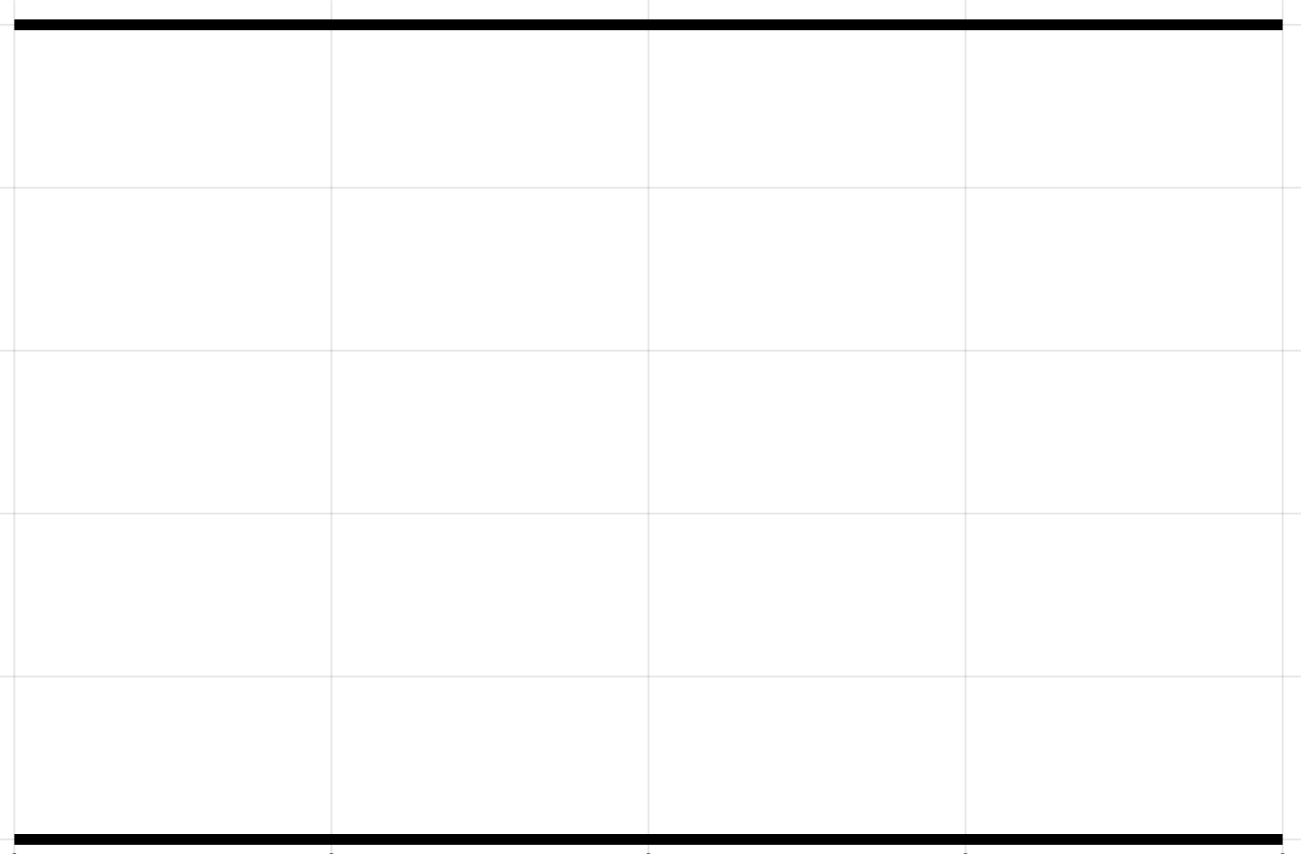
\includegraphics[scale=0.2]{figures/simple-road.png}
  \caption{\label{fig:simple-road} A straight road}
\end{figure}

\begin{figure}[ht]
  \centering
  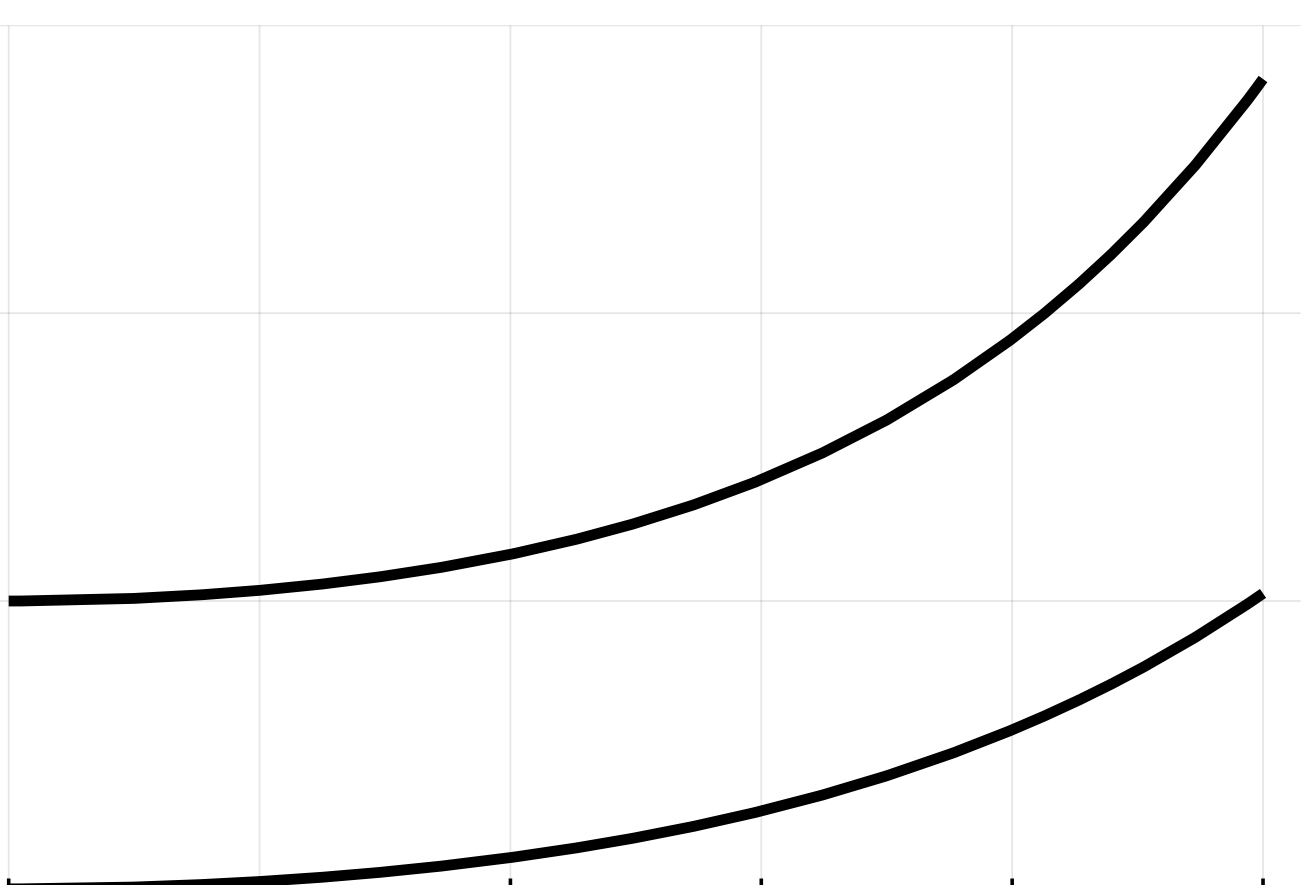
\includegraphics[scale=0.2]{figures/curved-road.png}
  \caption{\label{fig:curved-road} A curved road}
\end{figure}

\paragraph{Road Obstacles}

I have implemented two basic \texttt{Obstacle} types (\texttt{Rectangle} and \texttt{Circle}) allowing me to create regions of infeasible space within the valid road-space.

Infeasible space is then calculated by taking a sample of 500 points along a given curve $B$ and checking which (if any) lie within any of the obstacles.

A Bézier curve is then constructed using two applications of De Casteljau's algorithm (See Section~\ref{sec:decasteljau}) using values for $t$ derived from the subsample points. An illustration of this process can be seen in Figure~\ref{fig:ifspace-illustration}. The length of this curve is weighted and added to the overall fitness of the candidate solution. The stages progress as Follows:

\begin{enumerate}
  \item Curve and obstacle drawn
  \item Uniform sample of points chosen along curve
  \item Curve segment from origin to first infeasible point isolated
  \item Curve segment from last infeasible point to end position isolated
  \item Infeasible distance calculated as difference in length between original curve and two isolated segments
\end{enumerate}


A similar process is performed to determine how much of a curve passes too closely to an infeasible region, this is penalised with a separate, lower, weighting.

\begin{figure}
  \centering
  \begin{subfigure}[b]{0.44\textwidth}
    \centering
    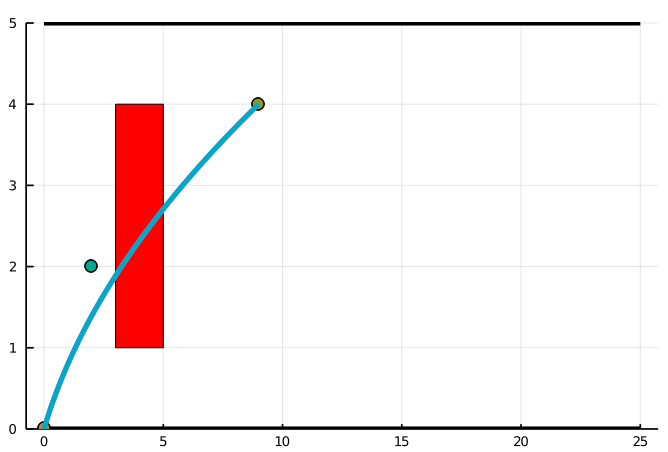
\includegraphics[width=\textwidth]{figures/obstacleavoidance-stage1.png}
    \caption{Stage 1}
  \end{subfigure}
  \begin{subfigure}[b]{0.44\textwidth}
    \centering
    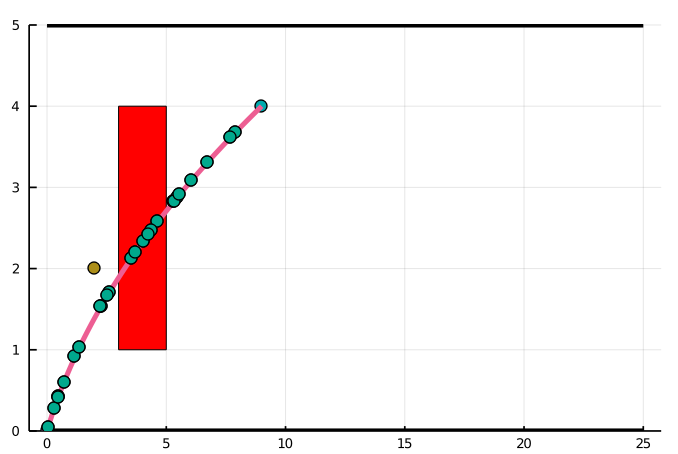
\includegraphics[width=\textwidth]{figures/obstacleavoidance-stage2.png}
    \caption{Stage 2}
  \end{subfigure}
  \begin{subfigure}[b]{0.44\textwidth}
    \centering
    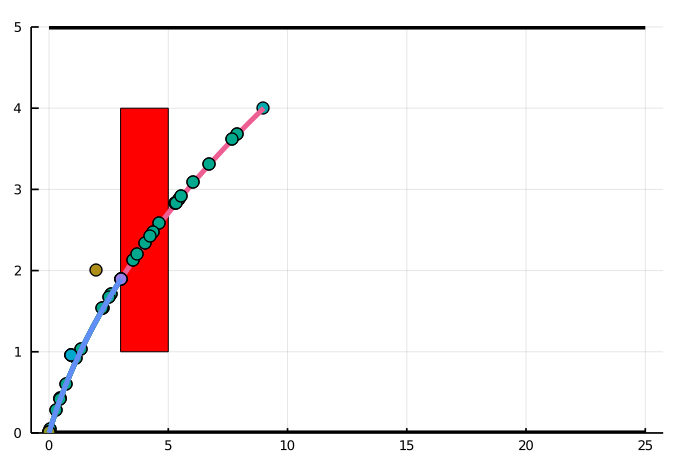
\includegraphics[width=\textwidth]{figures/obstacleavoidance-stage3.png}
    \caption{Stage 3}
  \end{subfigure}
  \begin{subfigure}[b]{0.44\textwidth}
    \centering
    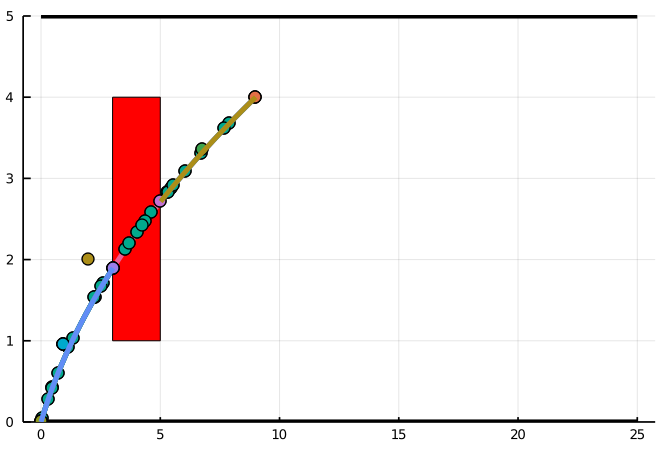
\includegraphics[width=\textwidth]{figures/obstacleavoidance-stage4.png}
    \caption{Stage 4}
  \end{subfigure}
  \begin{subfigure}[b]{0.44\textwidth}
    \centering
    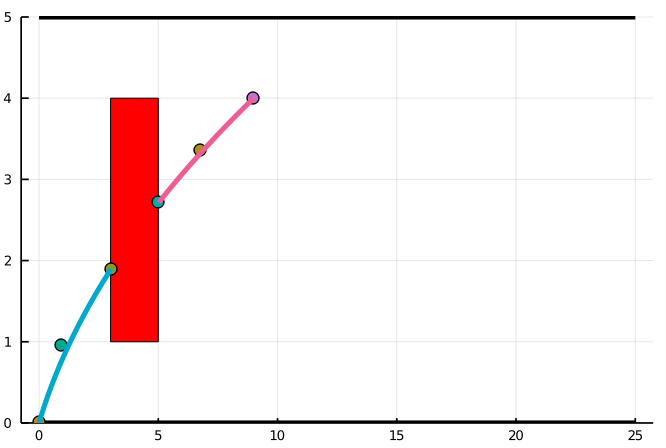
\includegraphics[width=\textwidth]{figures/obstacleavoidance-stage4-aux.png}
    \caption{Stage 5}
  \end{subfigure}
  \caption{\label{fig:ifspace-illustration} Illustration of finding infeasible section of curve}
\end{figure}\todo[inline]{Technically this infeasible distance calculation has very slightly changed in implementation, is it worth redoing or just leave as is?}

Now with the ability to calculate the length of a route as well as the distance it travels through/ too close to infeasible space, I can define my Fitness function:

\begin{multline}\label{eq:basefitness}
  \mathcal{F}(i) = \\
  L_{i} +\\
  \alpha \cdot \texttt{infeasible distance}(i) + \beta \cdot \texttt{high-proximity distance}(i)
\end{multline}\todo{formatting}

Where:
\begin{itemize}
  \item $L_{i}$ is the length of candidate $i$'s route
  \item \(\alpha\) and \(\beta\) are weighting parameters s.t.

        $\alpha > \beta > 1$

        therefore penalising infeasible distance harder than distance which is \textit{too close} to infeasible space, guiding the GA to prioritise avoiding infeasible space.
\end{itemize}

This function is inspired by Kala\cite{kalaOptimizationBasedPlanning2016} and proves to be a good basis for a naive single agent planner, futher augmentation is required to support multiple agents or variable velocity profiles.


\subsection{Genetic Operators}

The abstract goal of each genetic operator has already been discussed in Section~\ref{subsec:GAOps}. Here I will discuss their concrete implementation with respect to my task.

\subsubsection{Selection}
\label{subsec:approach:selection}

My selection procedure follows very closely to the method outlined in Section~\ref{subsec:GAOps}, relying on the fitness function to duplicate fit individuals, replacing the less fit ones with a certain chance or reasoning.

An example of ranked selection on a sample population can be seen in Figure~\ref{fig:selection_eg}

\begin{figure}
  \centering
  \begin{subfigure}[b]{0.44\textwidth}
    \centering
    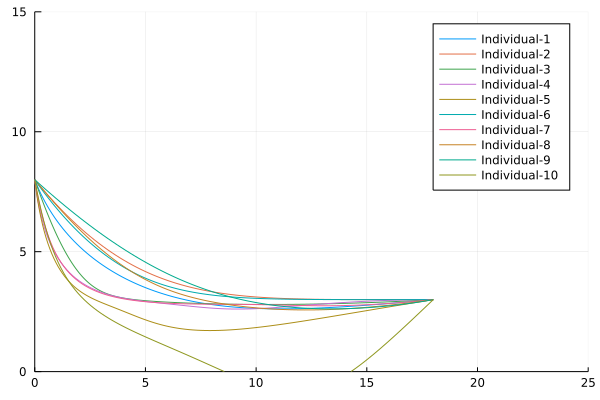
\includegraphics[width=\textwidth]{figures/init_pop.png}
    \caption{Initially generated population, size 10}
  \end{subfigure}
  \begin{subfigure}[b]{0.44\textwidth}
    \centering
    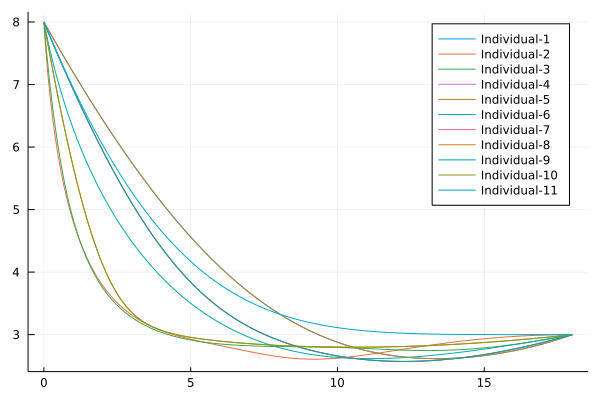
\includegraphics[width=\textwidth]{figures/post_selection_pop.png}
    \caption{Population after (ranked) selection procedure}
  \end{subfigure}
  \begin{subfigure}[b]{0.44\textwidth}
    \centering
    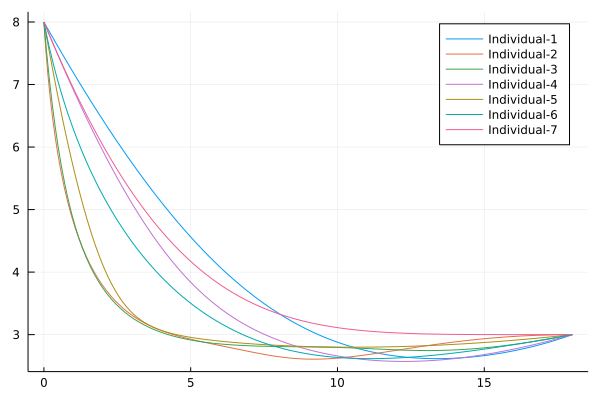
\includegraphics[width=\textwidth]{figures/post_selection_pop_unique.png}
    \caption{Population after (ranked) selection procedure, duplicates removed}
  \end{subfigure}
  \caption{\label{fig:selection_eg} Example of ranked selection}
\end{figure}


\subsubsection{Mutation}

The variants of the mutation operator that I have implemented are Uniform and Gaussian. Both attempt to achieve the same effect via different methods.

Abstractly, my mutation operators select a control point with a random probability and mutate within fixed bounds. These bounds are tied to the size and shape of the road.

In my Gaussian mutation operator, the range of $x$ values for the mutation of a randomly selected point $ p \in B = \{ p_{1}, \ldots, p_{n} \}, n\in \mathbb{Z}^{\geq 2 }$ are:

\begin{equation}
\mathcal{X} = \left[p_{1_{x}}, p_{n_{x}}\right], p_{1}, p_{n} \in B
\end{equation}

I.e. a mutated control point cannot lie before or after the start or end points respectively. The range of $y$ values a mutated point can take is within:

\begin{equation}
  \mathcal{Y} = \left[ - 1.3 \cdot \frac{b_{1}(\mathcal{X}_{1}) + b_{2}(\mathcal{X}_{2})}{2}, 1.3 \cdot \frac{b_{2}(\mathcal{X}_{1}) + b_{2}(\mathcal{X}_{2})}{2} \right]
\end{equation}

Meaning $-1.3$ times the average $y$ coordinate of the bottom road boundary to $1.3$ times the average of the top road boundary across the range of permitted $x$ values. $\pm 1.3$ was used after experimenting with values ranging from $\pm 2$ to $\pm 0.5$, 1.3 offers the procedure the chance to significantly affect the course of a route whilst, minimising the chance that the mutated route will be infeasible.

A pair standard deviations as previously outlined in the Background section are defined as:

\begin{equation}
\sigma_{x} = \frac{\mathcal{X}_{1}-\mathcal{X}_{2}}{10}
\end{equation}

\begin{equation}
\sigma_{y} = \frac{\mathcal{Y}_{1}-\mathcal{Y}_{2}}{10}
\end{equation}

A new point, $p'$, is then constructed as follows:

\begin{align}
  p'_{x}  &= \min(\max(\mathcal{N}(p_{x},\sigma_{x}),\mathcal{X}_{1}),\mathcal{X}_{2})\\
  p'_{y}  &= \min(\max(\mathcal{N}(p_{y},\sigma_{y}),\mathcal{Y}_{1}),\mathcal{Y}_{2})
\end{align}

Point $p \in B$ is then replaced with our new point $p'$.

The result of the operation being applied to a example curve can be seen in Figure~\ref{fig:gauss_mutation_eg}

\todo{Talk about implmentation of Uniform mutation operator }

\begin{figure}[ht]
  \centering
  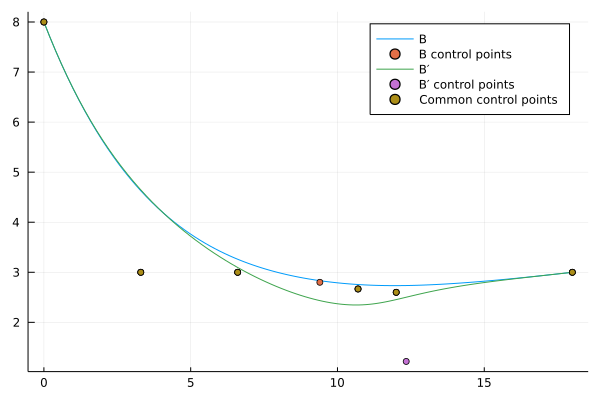
\includegraphics[scale=0.4]{figures/gauss_mutation_eg.png}
  \caption{\label{fig:gauss_mutation_eg} Example of Gaussian mutation on a Bézier curve}
\end{figure}

\subsubsection{Crossover}

Simple crossover is implemented as it is described in Section~\ref{subsec:GAOps}, two parents are randomly selected and exchange genotypic information about a random point. I have been careful not to choose a crossover point which splits a control point. The result of this operation is appended to the current population, only the top $n$ individuals are carried forward to the next generation.
Once used to create offspring, an individual cannot again participate in crossover, however, duplicate individuals created via the selection process may effectively reproduce multiple times.

The result of a single (simple) crossover operation can be seen in Figure~\ref{fig:crossover_eg}

\begin{figure}
  \centering
  \begin{subfigure}[b]{0.44\textwidth}
    \centering
    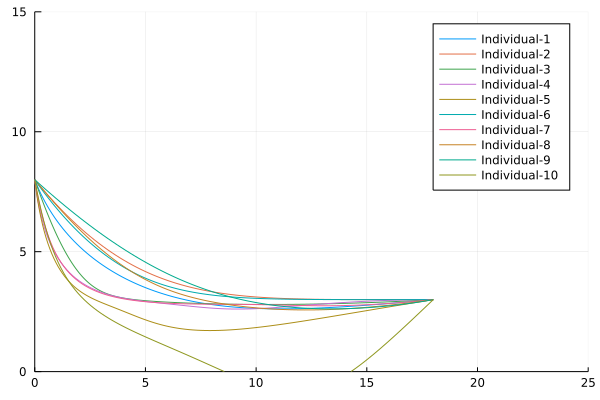
\includegraphics[width=\textwidth]{figures/init_pop.png}
    \caption{Initially generated population, size 10}
  \end{subfigure}
  \begin{subfigure}[b]{0.44\textwidth}
    \centering
    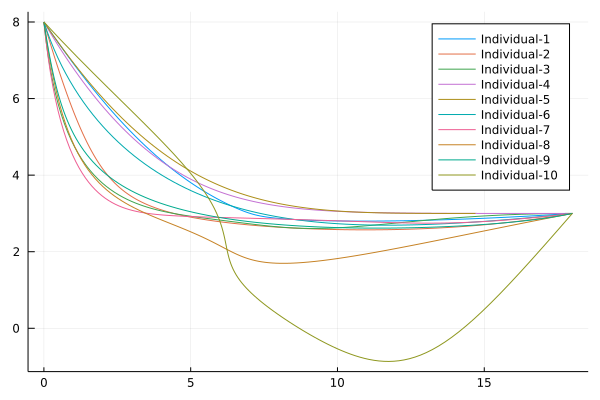
\includegraphics[width=\textwidth]{figures/post_crossover_pop.png}
    \caption{Population after crossover operation is applied}
  \end{subfigure}
  \caption{\label{fig:crossover_eg} Example of simple crossover}
\end{figure}

\section{Multi-agent Approach}
\label{sec:maa}

So far we have only concerned ourselves with planning a route through a road-space for a single agent. However, in the real world, roads are seldom occupied by a single vehicle and as such we must consider how to efficiently plan a set of routes for a set of agents between between a set of coordinate pairs, such that, our agents do not collide at any point in time.

There are different approaches we can take to this problem. \todo[inline]{refer to lit rev sections discussing approaches by Kala\cite{kalaOnroadIntelligentVehicles2016} and Cai \& Peng \cite{caiCooperativeCoevolutionaryAdaptive2002}}

My initial approach \todo{refer to ?Cai+Peng? as their approach was similar} to a collaborative planning system was somewhat inefficient. The system operated by planning routes for each agent sequentially, using a growing \textit{context} to keep track of the routes that had already been finalised. The first agent to be planned was not concerned with avoiding collisions, because, as far as it was concerned, there were no other agents in the system. Each subsequent agent checked if any of its candidate solutions intersected with any of the routes planned before, a very high penalty was applied to any routes with collisions.

This system was very inefficient with the final routes requiring a large number of checks to be carried out by my \texttt{bezInt} function, which itself suffered from \todo[inline]{verify this} exponential time (and space) complexity.

This system was improved upon by splitting the process over multiple threads, each agent being given a separate thread, communicating their most up-to-date plans via a shared array, $S$. Agent $i$ will store its current fittest route in $S[i]$, the calculation for fitness of any candidate checks for collisions with each route in $S$. This system may conduct more checks but it removes the problem of prioritising the first route to be planned and reduces the overall runtime of the system approximately proportionally to the number of threads available, an abstract view of the topology can be seen in Figure~\ref{fig:PCGA} with each agent $a_{k}, k \in [1,n]$ being mapped to a separate threaded instance of my GA planner. Each instance has access to the shared array which stores the fittest route after generation $i \in [1,m]$ with $m$ being the maximum number of generations for each agent.

Updates to the shared array happen as and when each thread reaches the end of a generation. This can mean that routes that terminate before others have to adapt less to other routes, but this trade-off cannot be avoided without instituting constant communication between threads, which in and of itself introduces overhead and slows down planning.

\begin{figure}
  \centering
\begin{tikzpicture}
  \node[] (V) {$\{ a_{1}, a_{2}, \ldots, a_{n} \} $};

  \node[draw, rectangle, above right= of V] (ga1) {$\texttt{GA}(a_{1})$};
  \node[draw, rectangle, below = of ga1] (ga2) {$\texttt{GA}(a_{2})$};
  \node[below = of ga2] (gael) {$\vdots$};
  \node[draw, rectangle, below = of gael] (gan) {$\texttt{GA}(a_{n})$};

  \coordinate[right = 0.12of ga1.east] (rGA1);
  \coordinate[right = 0.2cm of rGA1] (rrGA1);
  \coordinate[right = 0.12cm of gan.east] (rGAn);

  \node[below = 1cm of rGAn] (sa) {$\{ B_{a_{1}}^{i}, b_{a_{2}}^{i}, \ldots, B_{a_{n}}^{i} \}, i \in [1,m] $};
  \node[right = 2cm of gael] (res) {$\{ B_{a_{1}}^{m}, b_{a_{2}}^{m}, \ldots, B_{a_{n}}^{m} \}$};

  \node[draw=black, fit=(rGA1) (rGAn), label={[rotate=-90]center:\tiny Shared Array}]  {};
  \node[draw=red, fit=(ga1) (gan) (rrGA1)]  {};

  \draw[->] (V) -> (ga1);
  \draw[->] (V) -> (ga2);
  \draw[->] (V) -> (gael);
  \draw[->] (V) -> (gan);

  \draw[->] (sa) -> (rGAn);

  \draw[->] (ga1) -> (res);
  \draw[->] (ga2) -> (res);
  \draw[->] (gael) -> (res);
  \draw[->] (gan) -> (res);
\end{tikzpicture}
\caption{\label{fig:PCGA} Parallel Cooperative Genetic Algorithm abstract topology}
\end{figure}

\subsection{Collision Detection}
\label{subsec:col-detection}

Collision detection is one of the core obstacles to a viable cooperative route planner. You must be able to certify that your resulting set of routes do not collide at any point in time, else the entire system fails.

Simply detecting intersections is not enough as two routes can intersect but only collide if they pass through the same point at the same time. We therefore require some notion of time when realising our Bézier curve routes.

I made the assumption that each agent in my system travels at a uniform constant speed. To remove this assumption we would need to include a velocity-time profile in the genotype of each individual, this is an area for further research.

With this assumption, we can now say that two routes collide if they intersect and the distance from their respective origins and the point of intersection is the same (or below a threshold). We have now reduced this problem to finding a point of intersection between two Bézier curves, this is still a non-trivial task.

\subsubsection{Bézier Curve intersection}
\label{subsec:approach:bezInt}

The commonly employed technique for finding intersections between two $n$-degree Bézier curves is repeated recursive subdivision. Whilst it is possible to precisely calculate the point of intersection it is very difficult and computationally expensive and does not generalise well to $n$ degrees. For example, to numerically find the intersection two curves of degree 3 we must solve a $9^{th}$ order equation, producing unstable results. This is described by Bézout's theorem which states that two planar algebraic curves of degrees $d_{1}$ and $d_{2}$ will have up to $d_{1}d_{2}$ intersection points.\todo{cite this or remove it}

In their 2006 paper Yap\cite{yapCompleteSubdivisionAlgorithms2006} proposed an efficient method for finding the intersection of two Bézier curves through a 2 stage process surrounding repeated subdivision.

During development I attempted to use a Bézier curve library (\texttt{libbezier})\cite{Hermes2017} written for python but featuring a core written in Fortran, providing a C ABI. Julia, featuring interoperability with C and Fortran, allowed me to make direct calls to the Fortran subroutines and C functions. Ultimately, however, I encountered too many issues stemming from this library's inability to be run in parallel along with seemingly random segfaults which I struggled to diagnose through two levels of language abstraction (Fortran $\rightarrow$ C $\rightarrow$ Julia); this led me to write my own functions natively in Julia, although replicating the same accuracy as the nearly 4000 lines of Fortran proved challenging.

In order to speedup my Bézier intersection function I implemented a number of time saving measures:

\begin{enumerate}
  \item If the convex hulls of two curves $B_{1}$ and $B_{2}$ intersect, i.e. some amount of the area of the convex hull of $B_{1}$ ($CH(B_{1})$), lies inside the convex hull of $B_{2}$ ($CH(B_{2})$) then there may  be some intersection and as such, further checks are required. If however, this is not the case then (likely) the two curves do not intersect and the function can exit early.

        This is a simplified version of the logic presented by Yap in his \textit{Micro Phase} of intersection detection. However, in order to cover all edge cases and make this a reliable rule to follow a lot more precomputation is required (See Elementary curves \& curve coupling in~\cite{yapCompleteSubdivisionAlgorithms2006}).

        As such, I ended up removing this feature as the additional work required was too high for this project.\todo{phrasing? }
    \item I instead instituted a simpler heuristic using bounded boxes (See Section~\ref{subsec:back_boundedboxes}). Using the \texttt{Luxor} library\cite{JuliaGraphicsLuxorJl2021}, I was able to detect whether two bounded boxes intersected, if they did not, further checks can be skipped.\todo{Merge these first 2? }
  \item If two curve segments have already been checked for intersection, why bother checking them again?

        This question was solved by trading computation time for memory, by constructing a hash table linking curve pairs to a tuple containing the approximate values for $t$ representing the point of intersection (if present) and a boolean, when checking two curve sections, if they already exist in the hash table the remaining computation can be skipped with the pre-computed result returned instead.

        In most cases a check is performed at least twice. Given two candidate solutions for two distinct agents $B_{1}$ and $B_{2}$, when evaluating the fitness of $B_{1}$ it is checked for intersections with $B_{2}$ and equally when evaluating the fitness of $B_{2}$ $B_{2}$ is checked against $B_{1}$, thus buy storing the first result, the second check can be skipped.

        In reality, many curve segments are found repeatedly inside populations and as such many more duplicate checks can be skipped through this method.
  \item I implemented a recursion depth limit so as to introduce an upper bound in computation before the function returns false. Without this I found that often the checks would repeat until it was searching for intersections between infinitesimally small curve sections.

  \item I was also able to reduce the runtime of this function via the use of threading. Upon a subdivision two more threaded tasks are spawned and the lazy disjunction of their results returned. The optimal case for this approach is that the intersection occurs early on in the curve as the task results must be fetched sequentially in the order that they were spawned. \todo{remove this sentence?}

\end{enumerate}

My method keeps track of the divisions made and using this keeps track of the $t$ value which maps $P_{n}$ from the subcurve to the initial curve. The values of $t$ are then returned if a intersection is found, this allows for the distances from the origin points to the point of intersection to be easily calculated using De Casteljau's algorithm along with my function for finding the length of a Bézier curve.

An illustration of the recursive subdivision method described above can be seen in Figure~\ref{fig:bezIntIllustration}

\begin{figure}
\begin{turn}{90}
\begin{tikzpicture}[level/.style={sibling distance = 10cm/#1,
  level distance =4cm}]
  \node [] {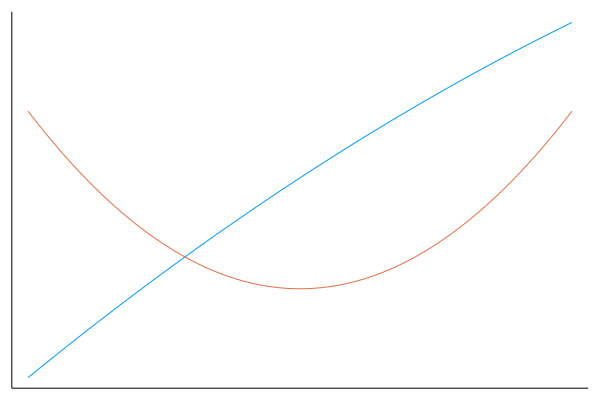
\includegraphics[scale=0.25]{images/bezint-1.png}}
  child{
    node [] {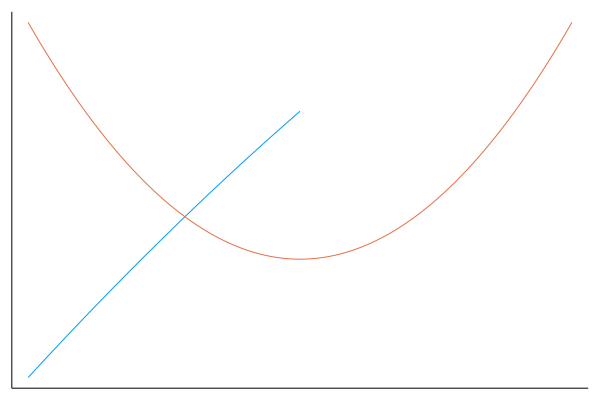
\includegraphics[scale=0.25]{images/bezint-2:1.png}}
    child{
      node [] {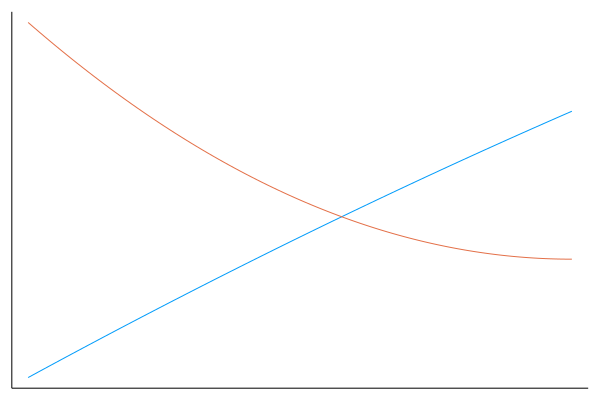
\includegraphics[scale=0.25]{images/bezint-3:1, 3.png}}
      %child{
      %  node [] {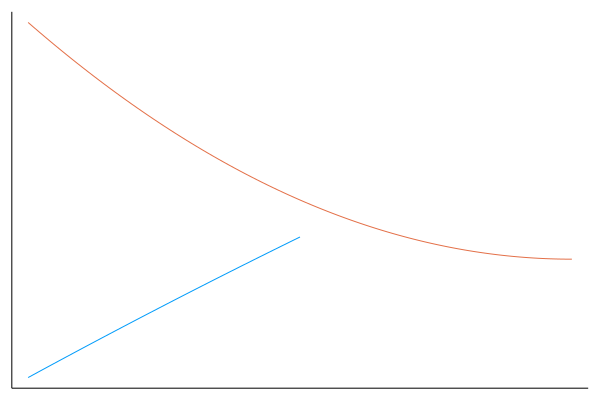
\includegraphics[scale=0.25]{images/bezint-4:1, 3, 1.png}}
      %  %child{
      %  %  node [] {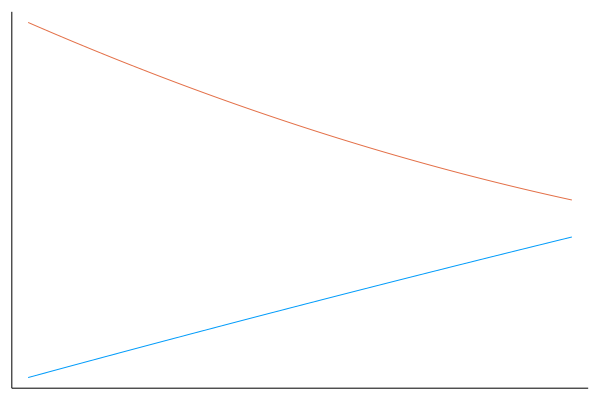
\includegraphics[scale=0.25]{images/bezint-5:1, 3, 1, 3.png}}
      %  %}
      %  %child{
      %  %  node [] {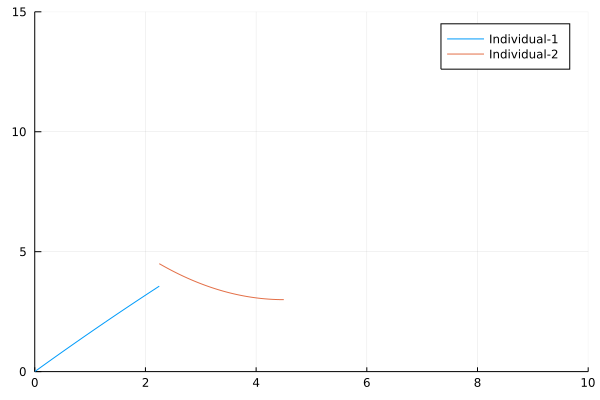
\includegraphics[scale=0.25]{images/bezint-5:1, 3, 1, 4.png}}
      %  %  child{
      %  %    node [] {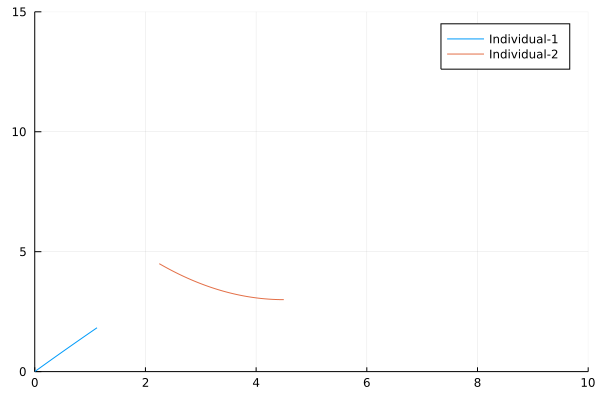
\includegraphics[scale=0.25]{images/bezint-6:1, 3, 1, 4, 1.png}}
      %  %  }
      %  %  %child{
      %  %  %  node [] {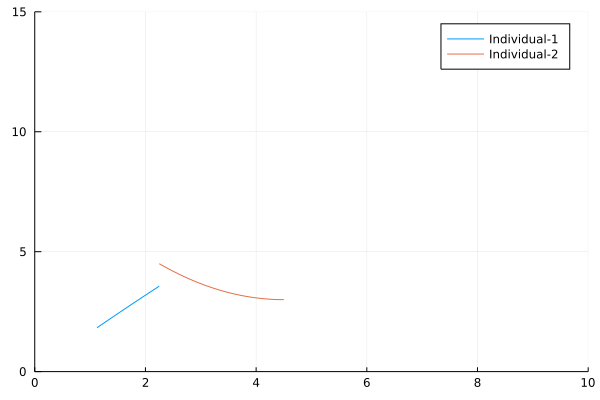
\includegraphics[scale=0.25]{images/bezint-6:1, 3, 1, 4, 2.png}}
      %  %  %  %child{
      %  %  %  %  node [] {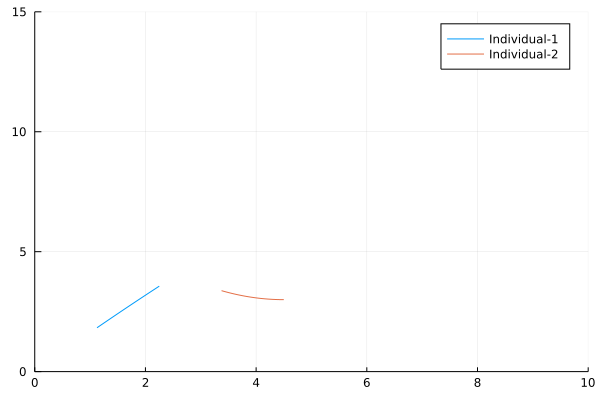
\includegraphics[scale=0.25]{images/bezint-7:1, 3, 1, 4, 2, 3.png}}
      %  %  %  %}
      %  %  %  %child{
      %  %  %  %  node [] {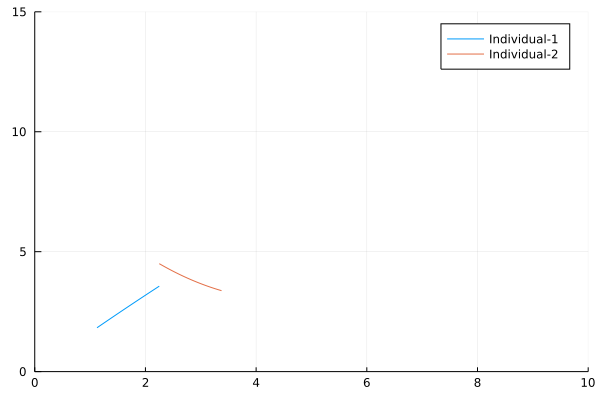
\includegraphics[scale=0.25]{images/bezint-7:1, 3, 1, 4, 2, 4.png}}
      %  %  %  %  child{
      %  %  %  %    node [] {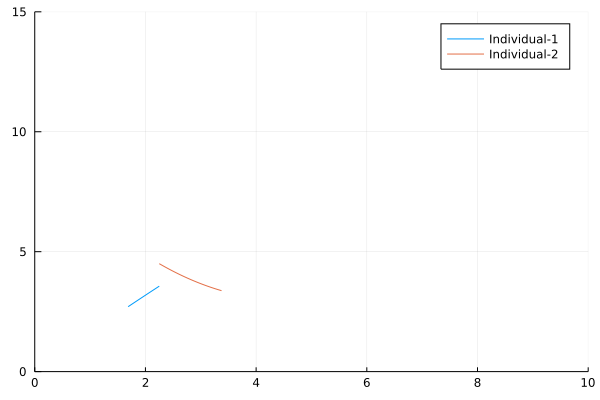
\includegraphics[scale=0.25]{images/bezint-8:1, 3, 1, 4, 2, 4, 1.png}}
      %  %  %  %  }
      %  %  %  %  child{
      %  %  %  %    node [] {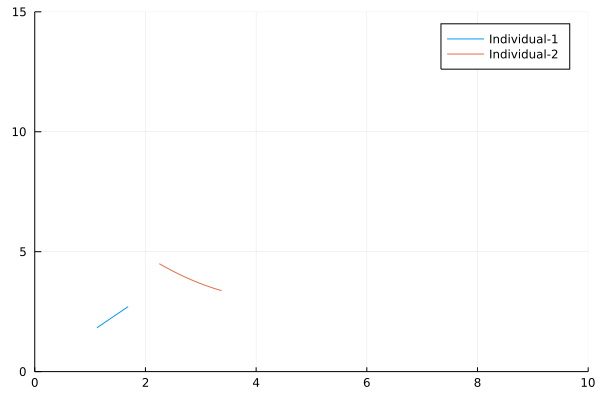
\includegraphics[scale=0.25]{images/bezint-8:1, 3, 1, 4, 2, 4, 2.png}}
      %  %  %  %  }
      %  %  %  %}
      %  %  %}
      %  %}
      %}
      %child{
      %  node [] {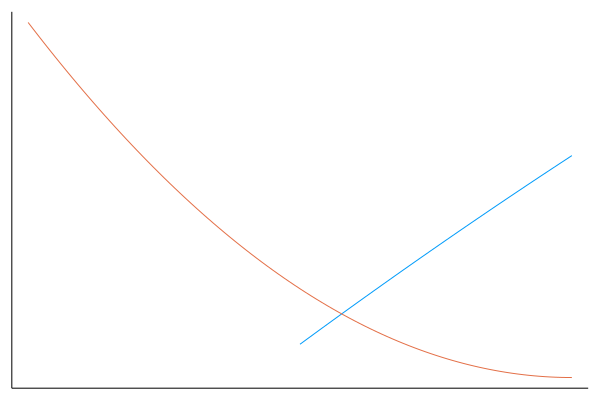
\includegraphics[scale=0.25]{images/bezint-4:1, 3, 2.png}}
      %  %child{
      %  %  %node [] {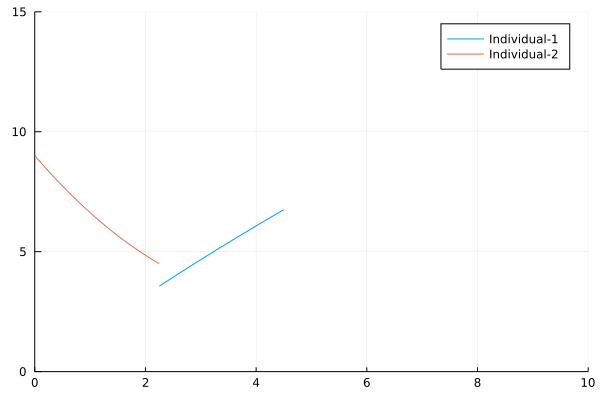
\includegraphics[scale=0.25]{images/bezint-5:1, 3, 2, 3.png}}
      %  %  %child{
      %  %  %  node [] {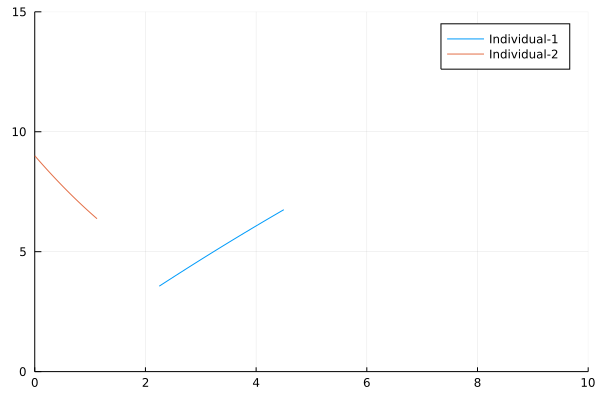
\includegraphics[scale=0.25]{images/bezint-6:1, 3, 2, 3, 3.png}}
      %  %  %}
      %  %  %child{
      %  %  %  node [] {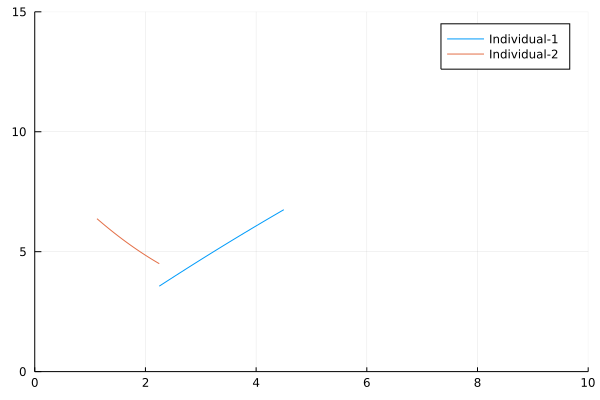
\includegraphics[scale=0.25]{images/bezint-6:1, 3, 2, 3, 4.png}}
      %  %  %  %child{
      %  %  %  %  node [] {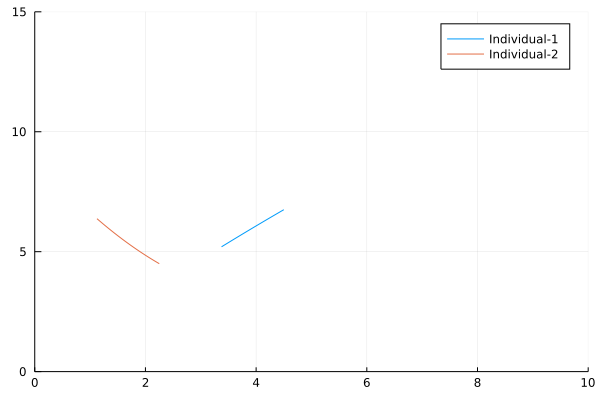
\includegraphics[scale=0.25]{images/bezint-7:1, 3, 2, 3, 4, 1.png}}
      %  %  %  %}
      %  %  %  %child{
      %  %  %  %  node [] {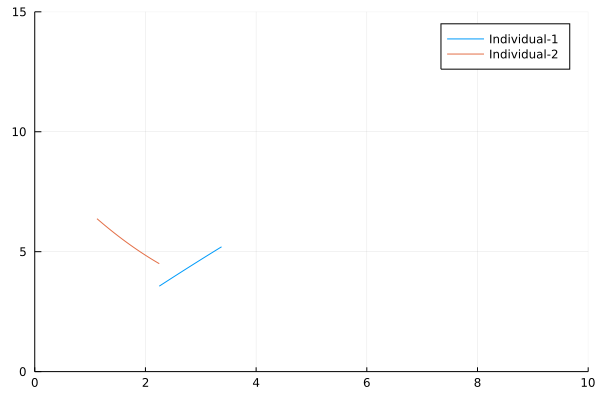
\includegraphics[scale=0.25]{images/bezint-7:1, 3, 2, 3, 4, 2.png}}
      %  %  %  %  child{
      %  %  %  %    node [] {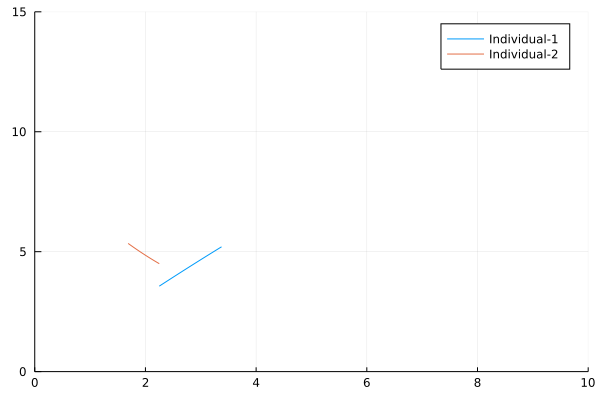
\includegraphics[scale=0.25]{images/bezint-8:1, 3, 2, 3, 4, 2, 3.png}}
      %  %  %  %  }
      %  %  %  %  child{
      %  %  %  %    node [] {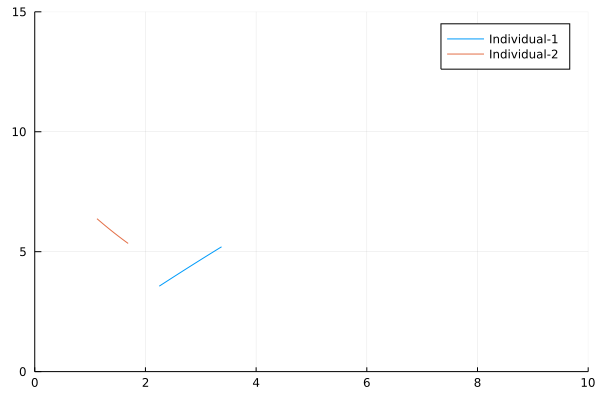
\includegraphics[scale=0.25]{images/bezint-8:1, 3, 2, 3, 4, 2, 4.png}}
      %  %  %  %  }
      %  %  %  %}
      %  %  %}
      %  %}
      %  %child{
      %  %  %node [] {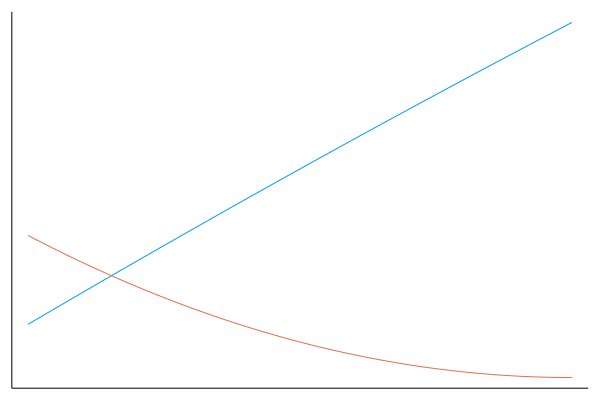
\includegraphics[scale=0.25]{images/bezint-5:1, 3, 2, 4.png}}
      %  %  %child{
      %  %  %  node [] {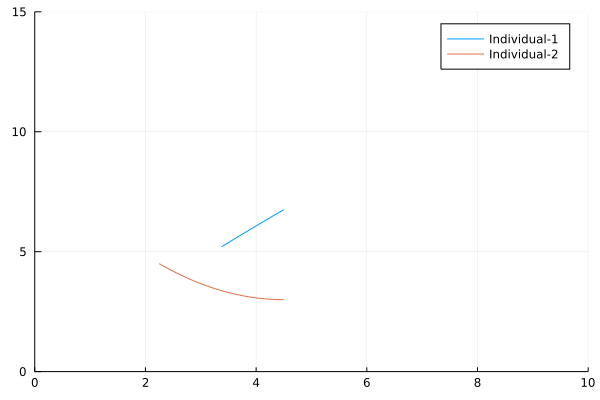
\includegraphics[scale=0.25]{images/bezint-6:1, 3, 2, 4, 1.png}}
      %  %  %}
      %  %  %child{
      %  %  %  node [] {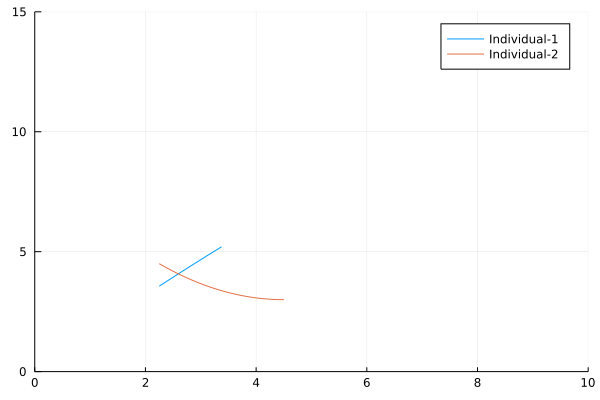
\includegraphics[scale=0.25]{images/bezint-6:1, 3, 2, 4, 2.png}}
      %  %  %  %child{
      %  %  %  %  node [] {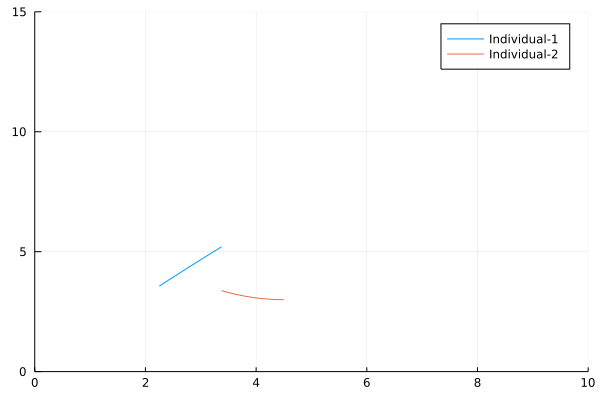
\includegraphics[scale=0.25]{images/bezint-7:1, 3, 2, 4, 2, 3.png}}
      %  %  %  %}
      %  %  %  %child{
      %  %  %  %  node [] {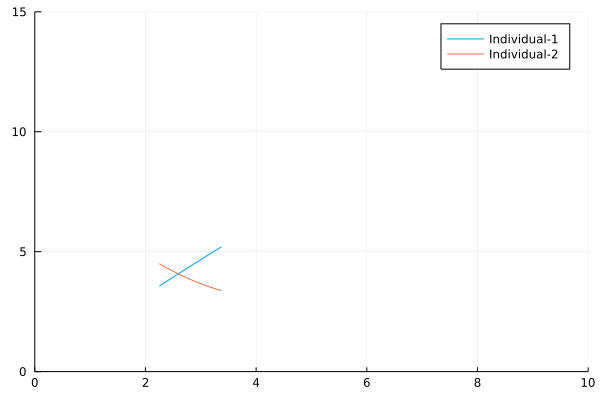
\includegraphics[scale=0.25]{images/bezint-7:1, 3, 2, 4, 2, 4.png}}
      %  %  %  %}
      %  %  %}
      %  %}
      %}
    }
    child{
      node [] {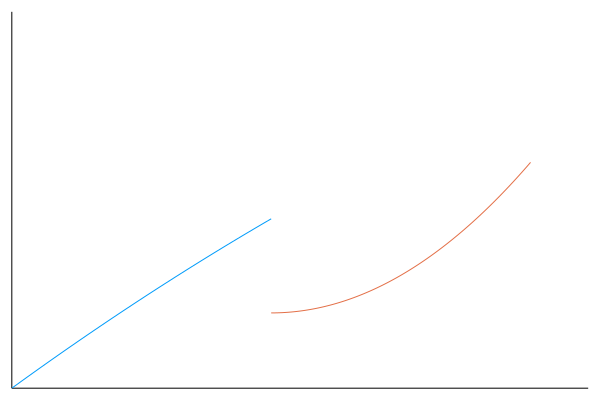
\includegraphics[scale=0.25]{images/bezint-3:1, 4.png}}
      %child{
      %  node [] {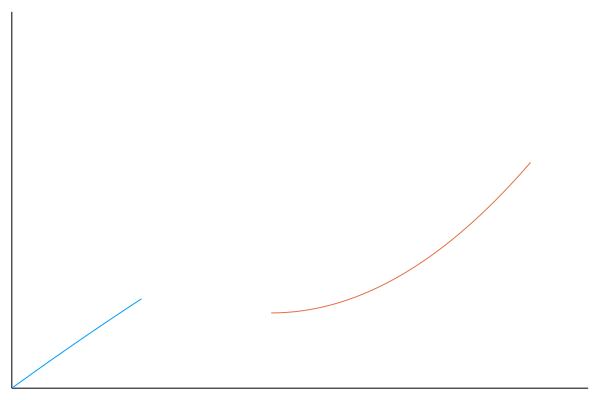
\includegraphics[scale=0.25]{images/bezint-4:1, 4, 1.png}}
      %}
      %child{
      %  node [] {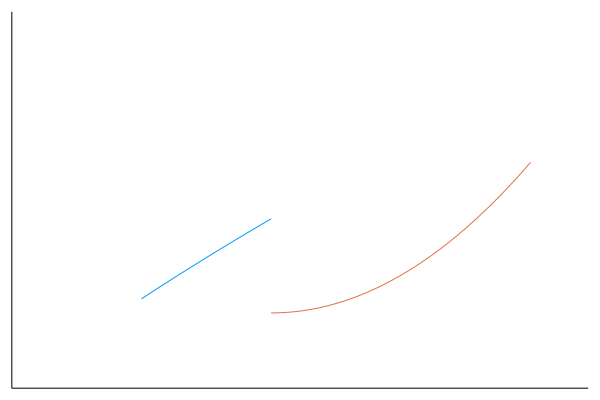
\includegraphics[scale=0.25]{images/bezint-4:1, 4, 2.png}}
      %  %child{
      %  %  %node [] {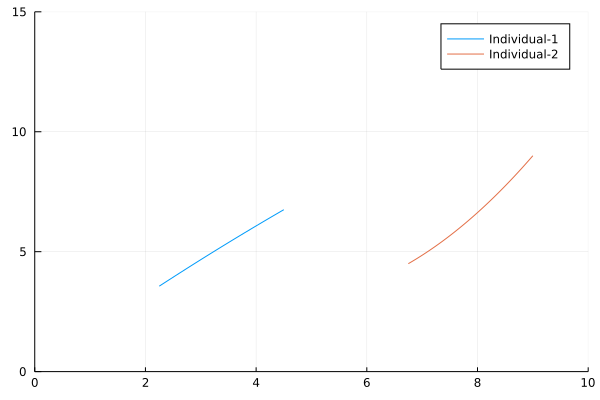
\includegraphics[scale=0.25]{images/bezint-5:1, 4, 2, 3.png}}
      %  %}
      %  %child{
      %  %  %node [] {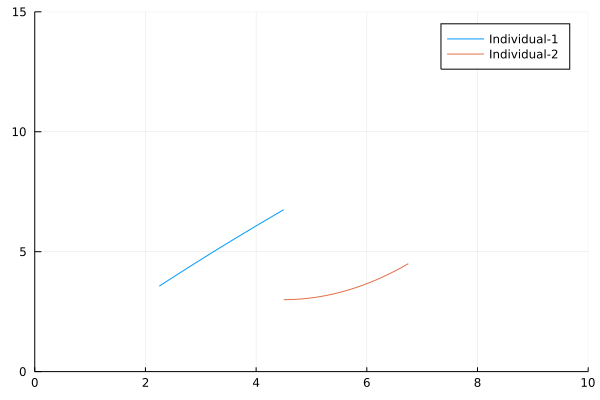
\includegraphics[scale=0.25]{images/bezint-5:1, 4, 2, 4.png}}
      %  %  %child{
      %  %  %  node [] {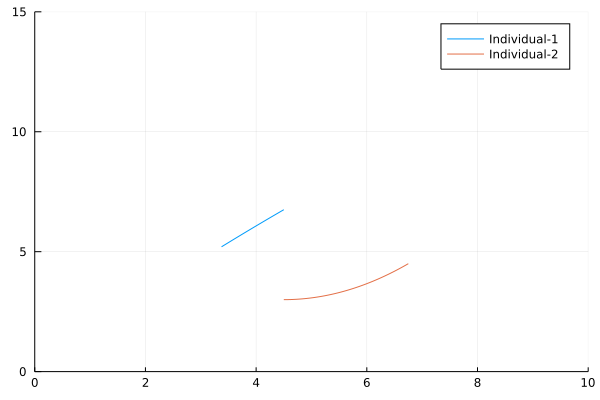
\includegraphics[scale=0.25]{images/bezint-6:1, 4, 2, 4, 1.png}}
      %  %  %}
      %  %  %child{
      %  %  %  node [] {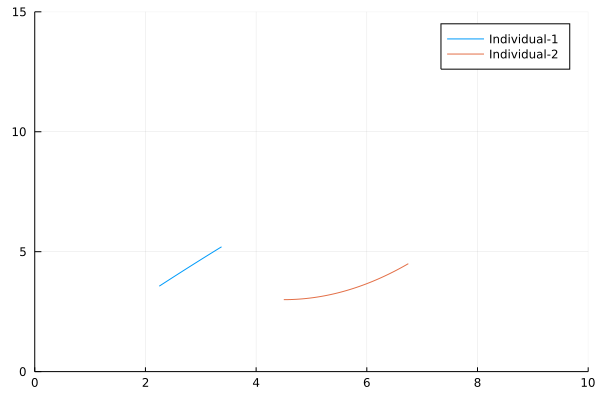
\includegraphics[scale=0.25]{images/bezint-6:1, 4, 2, 4, 2.png}}
      %  %  %}
      %  %}
      %}
    }
}
  child{
    node [] {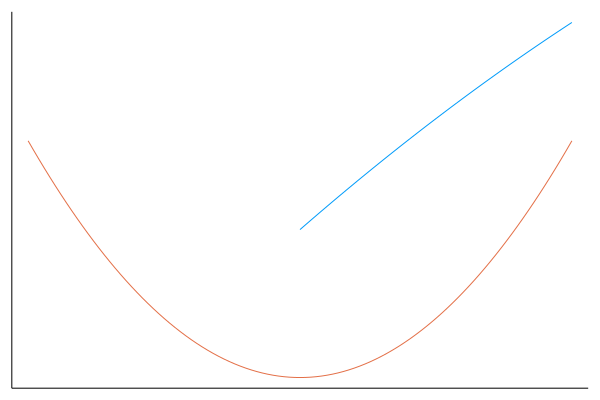
\includegraphics[scale=0.25]{images/bezint-2:2.png}}
    child{
      node [] {\includegraphics[scale=0.25]{images/bezint-3:2, 3.png}}
      %child{
      %  node [] {\includegraphics[scale=0.25]{images/bezint-4:2, 3, 3.png}}
      %}
      %child{
      %  node [] {\includegraphics[scale=0.25]{images/bezint-4:2, 3, 4.png}}
      %}
    }
    child{
      node [] {\includegraphics[scale=0.25]{images/bezint-3:2, 4.png}}
      %child{
      %  node [] {\includegraphics[scale=0.25]{images/bezint-4:2, 4, 3.png}}
      %  %child{
      %  %  %node [] {\includegraphics[scale=0.25]{images/bezint-5:2, 4, 3, 1.png}}
      %  %}
      %  %child{
      %  %  %node [] {\includegraphics[scale=0.25]{images/bezint-5:2, 4, 3, 2.png}}
      %  %  %child{
      %  %  %  node [] {\includegraphics[scale=0.25]{images/bezint-6:2, 4, 3, 2, 3.png}}
      %  %  %}
      %  %  %child{
      %  %  %  node [] {\includegraphics[scale=0.25]{images/bezint-6:2, 4, 3, 2, 4.png}}
      %  %  %}
      %  %}
      %}
      %child{
      %  node [] {\includegraphics[scale=0.25]{images/bezint-4:2, 4, 4.png}}
      %}
    }
  }
  ;

%  \node [below left = of p2-1] (p3-13) {\includegraphics[scale=0.25]{images/bezint-3:1, 3.png}};
%  \node [below right = of p2-1] (p3-14) {\includegraphics[scale=0.25]{images/bezint-3:1, 4.png}};
%
%  \node [below left = of p2-2] (p3-23) {\includegraphics[scale=0.25]{images/bezint-3:2, 3.png}};
%  \node [below right = of p2-2] (p3-24) {\includegraphics[scale=0.25]{images/bezint-3:2, 4.png}};


\end{tikzpicture}


\end{turn}
\caption{\label{fig:bezIntIllustration} Illustration of Bezier Intersection recursive subdivision method (Recursion depth =2)}
\end{figure}

\section{Macro-Level Planning} \todo{Title?}

The next stage in development is to attempt to implement the wrapper to solve Problem~\ref{prob:Spec} using the solution to Problem~\ref{prob:sub1}. I.e. to go from planning for multiple agents in a single section of road to planning for multiple agents across a network of interconnected roads.

\subsection{Road Graph Construction }

As specified in Problem~\ref{prob:Spec}, we require a description of the road space as a graph, $\mathcal{R}= (V,E)$ of intersections, $V$ and road segments $E$\todo[inline]{Should I define it as $\mathcal{R} = (I, R)$?}
.

This is a malleable definition allowing for a lot of information to be encapsulated whilst maintaining an abstract canonical description compatible with a swathe of mathematics through graph theory.\todo[inline]{wordy?}

I decided to use a mixture libraries to construct my road network: \texttt{Graphs.jl}\cite{JuliaAtticGraphsJl2021}, \texttt{LightGraphs.jl}\cite{Bromberger17}  and \texttt{SimpleWeightedGraphs.jl}\cite{JuliaGraphsSimpleWeightedGraphsJl2021}. The graph structures found in \texttt{Graphs.jl} allow for a lot of data (The entirety of the \texttt{Road} structure can be stored as edge metadata) to be encapsulated but do not offer the same functionality as those found in \texttt{LightGraphs.jl}, \texttt{SimpleWeightedGraphs.jl} utilises the \texttt{LightGraphs.jl} format but allows for weighted edges when applying the various standard graph-based algorithms (including Dijkstra), as such I created my own helper functions to convert between the two formats, which is a relatively simple process of filtering data into a new, more restrictive, structure.

In the simplified weighted digraph format, the edges are weighted by their length. Going forward it would be possible to incorporate more advanced heuristics into this, mimicking the method by which applications such as Google Maps plan routes. This could include congestion, road surface quality, known planned road obstruction such as maintenance or a predicted large influx of vehicles, for example the exodus of people from a large sports arena.

A visualisation of this format can be seen in Figure~\ref{fig:demoGraph} with edge names and their respective weights labelled.


\begin{figure}[ht]
  \centering
  \includegraphics[scale=0.4]{figures/demoGraph.png}
  \caption{\label{fig:demoGraph} Example Road Graph, edge names take the form $e$<start><end>: <edgeweight> }
\end{figure}


With the graph constructed the next stage is to plan what I will refer to as the \textit{macro} routes, i.e. the set of edges the agent must travel along $\{e_{1},\ldots,e_{m}\} \subseteq E$ to reach its destination intersection, $d \in V$.

\subsection{Macro-Route planning}

Macro-route planning, as described in Problem~\ref{prob:Spec}, is the process of taking a set of intersection pairs corresponding to agents and producing the set of edges which connect the vertex pairs in the shortest distance. This task is almost the exact specification for Dijkstra's algorithm~\cite{dijkstra1959note} for finding shortest paths in a connected digraph and as such this is the algorithm I employed to solve it.

The \texttt{LightGraphs.jl} library already implements this algorithm and the weighted element is incorporated by the \texttt{SimpleWeightedGraphs.jl} sub-library. As previously mentioned, the edges of my road-graph are weighted by their lengths.

For example the following construction of inputs for Problem~\ref{prob:Spec} over the graph seen in Figure~\ref{fig:demoGraph}:

\begin{align*}
  A &= \{ a_{1},a_{2},a_{3},a_{4} \} \\
  \mathcal{V} &= [ (1,4), (4,2), (1,4), (3,5) ]
\end{align*}

Would yield the following abstract routes for the agents:


\begin{align*}
  P &= \{ \\
  a_{1} &\mapsto \{ 1,3,2,5,4 \}, \\
  a_{2} &\mapsto \{ 4,5,2 \}, \\
  a_{3} &\mapsto \{ 1,3,2,5,4 \} ,\\
  a_{4} &\mapsto \{ 3,2,5 \} \\
          \}
\end{align*}

The next stage in the process is to group these agents into \textit{planning groups} i.e. groups in which agents will occupy the same road at the same time thus requiring cooperative planning.

\subsection{Agent Grouping}

When planning for multiple agents across multiple road spaces, routes may share the same stretch of road during route execution.

In the above example, it is trivial to see that agents $a_{1}$ and $a_{3}$ will share the same road at each stage of their route as they are following the same abstract path. We however, must also be able to determine whether agents $a_{1}$ and $a_{4}$ share road $e25$, it occurs in both of their routes but one agent may have left that stretch of road before the other enters.

This problem is solved using the algorithm seen in Algorithm~\ref{alg:pathgrouping}\feedback{do I need to make it more obvious that these algorithms are my own work? Are they clear enough?}
. For instance, on the example input above, we would expect to see the following grouping:

\begin{align*}
  (3,2) &\mapsto \{ \{ a_4,a_1,a_3 \}  \}, \\
  (4,5) &\mapsto \{ \{ a_2 \}  \}, \\
  (2,5) &\mapsto \{ \{ a_3,a_1 \}, \{ a_4 \}   \}, \\
  (5,2) &\mapsto \{ \{ a_2 \}  \} , \\
  (1,3) &\mapsto \{ \{ a_3,a_1 \}  \} , \\
  (5,4) &\mapsto \{ \{ a_3,a_1 \}  \}
\end{align*}

Where you can see $a_{4}$ occupies edge $e25$ at a time separate from agents $a_{1}$ and $a_{3}$.

\begin{algorithm}
  \caption{Path Grouping, \texttt{getPathGroupings} }\label{alg:pathgrouping}
  \KwIn{
  \begin{itemize}
    \item a road network graph $\mathcal{R} = (V,E)$
    \item a macro-path for each agent, $P$.
  \end{itemize}
}
Initialise map of roads, \texttt{roads}

\For{each road, $r \in E$}{
  \texttt{roads}[$r$] = [  ] \tcp*{Initialise list of agent groups}
}

\For{each agent's macro-path, $i \in P$}{
    Construct a running total of distance for each edge.

    \For{each edge, $e \in E$ in the macro-path}{

      \tcp*{Initialise routes sharing edge $e$ with agent $i$}
      microPlanAgents = [ i ]

      \For{each other agent's macro-path, $o \in P\backslash i$}{
        \If{$e \in o$ }{ \tcp*{routes $i$ and $o$ share an edge ($e$) at some point}

          \uIf{length of $i$ from origin to end of $e$ $>$ length of $o$ from origin to start of $e$}{
            \tcp*{routes $i$ and $o$ occupy the edge $e$ at the same time}
              append(microPlanAgents, o)
          }\Else{
            \tcp*{route $i$ exits edge $e$ before $o$ enters}
            continue
          }
        }
      }
      append(\texttt{roads}[$e$], microPlanAgents)
    }
  }

  \KwRet{roads}\tcp*{A map of edges to a list of lists of routes sharing that edge at the same time.}
\end{algorithm}

Once these grouping have been constructed, the next stage is to plan the low-level curves representing the paths each agent must take through each road segment, avoiding any agents it shares a given road segment with.

\subsection{Multi-agent route planning}\todo{title?}

This process is a wrapper around the previously implemented parallel planner described in~\ref{sec:maa}. It follows the algorithm outlined in Algorithm~\ref{alg:mrp}.

\begin{algorithm}
  \caption{Macro-route planner}\label{alg:mrp}
  \KwIn{
    \begin{itemize}
      \item set of start-goal pairs for each agent, $\mathcal{V}$
      \item a graph representing a road network, $\mathcal{R}$
    \end{itemize}
  }

  $P$ = $djikstraShortestPath(\mathcal{R},\mathcal{V})$

  pathGroupings = $\texttt{getPathGroupings}(\mathcal{R}, P)$

  routes = [] \tcp*{initialise routes array as list of paths through each road segment specified by macro-route in $P$}

  \For{each macro-path, $p\in P$}{
    \For{each edge $e \in p$}{
      concurrentAgentSets = pathGroupings[$e$]

      \For{concurrentAgents $\in$ concurrentAgentSets}{

        construct start and goal positions for each agent. This process requires further thought/ research \textbf{better way to talk about this?}

        paths = parallelPlanner(startPositions, goalPositions, $e$) \tcp*{Parallel planner, solution to Problem~\ref{prob:sub1}}

        \For{each agent $a_{i} \in \mathcal{V}$}{
          append(routes[$i$], paths[$i$])
        }

      }
    }
  }

  \Return{routes}

\end{algorithm}\todo{phrasing about s/e position calculation on alg~\ref{alg:mrp}}


My approach vastly simplifies the problem of intersection navigation and linking the routes between road segments, essentially assuming all road segments are sections of a single long road which line up exactly. Papers such as ``Automated Optimization of Intersections Using a Genetic Algorithm'' by Cruz-Piris et al.\cite{cruz-pirisAutomatedOptimizationIntersections2019} begin to tackle this problem through the use of cellular automata (building on the work of Maerivoet and De Moor\cite{maerivoetCellularAutomataModels2005}\todo[inline]{necessary?}
) and GAs (See Section~\ref{subsec:lit_rev-GACoopRoutes}) but substantial work would be required to link our two systems together.



\section{Language Choice}\todo[inline]{decide whether to remove this, I am thinking yes but last para is interesting, maybe move to evaluation}

I have chosen to implement my approach using the Julia language project\cite{JuliaProgrammingLanguage}.

Julia is a relatively new language first developed in 2012 by Jeff Bezanson, Stefan Karpinski and Viral Shah. It is a multi-paradigm language allowing for functional, object oriented (OO) and meta programming approaches to problems. I will mainly be using it for it's functional and OO capabilities.

Julia operates using multiple dispatch similar to languages such as Haskell. It interoperates with C and Fortran codebases without the need of middle-man bloat. This fact allows it to utilise the extensive high performance C libraries for floating point operations. Julia is eagerly evaluated, uses a Just in time compiler and has a garbage collector.

Julia features a syntax similar to both Python and Matlab with performance on par with C. As I am already very familiar with python and have studied functional programming in a number of modules; I found this language very quick and intuitive to learn and the resulting code to be clean, idiomatic and fast.

\todo{revise this para}A real-world deployment of a system based on my research would undoubtedly be required to run on small, relatively low performance, embedded systems and as such Julia may not be appropriate here. A language such as C or Rust may be used instead.

Julia also has distributed computation facilities. This sort of functionality could be extremely useful in a system such as mine as it could allow for computation to be spread across the agents themselves, removing the need for a central planning centre which could be a single point of failure.



%TC:macro \todo 1


%%% Local Variables:
%%% mode: latex
%%% TeX-master: "report"
%%% End:

\chapter{Evaluation}\label{chap:Eval}
This section of my report contains many 3 dimensional plots. I have included static captures and attempted to capture them at angles which demonstrate the points I am making. I have hosted all 3D plots seen below and they can be found indexed \href{https://barrett370.github.io/Y4-Diss/posts/figures}{here:} https://barrett370.github.io/Y4-Diss/posts/figures. I feel the data is better understood and expressed using these interactive plots.

\todo{Insert more headings to break up this section}

\section{Genetic Algorithms}
\label{sec:eval:GAs}

The core of my approach to solving the problems outlined in Chapter~\ref{chap:Intro} was creating a Genetic algorithm to evolve populations of candidate routes, returning the fittest once the termination criteria are met.

GAs are transparent but stochastic approaches to optimisation problems. As such, it is much easier to examine the operations and decisions they make compared with \textit{black box} approaches such as neural networks, however due to their random nature, it can be difficult to predict their exact behaviour and results can differ greatly from run to run if the number of generations or population size is too low.

Whilst a poor choice of training data can lead to unintended/ unpredictable behaviour from approaches like neural networks, they have the advantage that most of their compute time is used when constructing the initial model, subsequent usage of these models requires little compute time. Whereas, GAs must run the entirety of the \textit{learning} process from scratch whenever a new route or set of routes is required. In an application where the system sees a high number of unique requests, this compute time can quickly amount to much longer than the training time for a neural network.

\subsection{Genetic Operator Performance}

During development I implemented two different operators in each category, but there are many other approaches proposed in academic literature. Given more time, I would have liked to implement more and present a more empirical evaluation of each.

\subsubsection{Selection}

In a single generation, over three populations of 15 individuals, my ranked selection operator ran 3 times totalling $75.1\mu s$ or an average of $25 \mu s$ per run, a negligible amount of time relative to the overall runtime.

As you can see in Figure~\ref{fig:selection_eg}, my ranked selection operator performs its task well, removing the obviously less fit individuals in favour of more copies of  fitter ones. This can be seen by the removal of the line that dips below the $x$ axis (in this example the bottom road boundary was defined as $b_{1}(x) = 0 $) and the fact that duplicate routes are found as indicated by the 3rd graph of unique routes showing fewer individuals than the second.

Ranked selection compared with fitness proportional (roulette wheel selection) is much more predictable, it may not explore as much of the search space but it is more likely to thoroughly explore a single area. Most other selection operators seem to focus on maintaining a diverse population so as to not get stuck in local minima.

\subsubsection{Mutation}

The mutation operators I implemented were Uniform and Gaussian.

I found Gaussian to perform better in cases where a route may be close to optimal in the phenotypic space, i.e. with minimal changes to trajectory, it would be optimal. In such cases the genotypic fitness may not accurately represent this, a route that collides with another or passes through infeasible space will suffer from a large genotypic fitness penalty possibly encouraging it to be removed from the \textit{gene pool}. Gaussian mutation, preferring mutated points closer to their initial position can be effective as moving such routes closer to the optima.

However, in cases where the initial population generation has created all routes far from the optimal, Gaussian mutation can struggle to generate mutated points extreme enough to direct the GA towards the minima.

Part of the problem with Gaussian mutation, and mutation in general on $n$-degree Bezier curves, is that even a relatively major control point movement may cause only minor changes to the overall trajectory of the curve in cases where $n$ is high.

An example of a relatively large control point mutation leading to a minor direction change can be seen in Figure~\ref{fig:gauss_mutation_eg}.

It is possible that an approach incorporating a form of Simulated Annealing could help to broadly explore the search space in early generations before refining solutions in a found minima in latter generations. This could operate by applying a different mutation operator such as Uniform mutation in the first 60\% of generations before swapping to Gaussian when we would expect our algorithms to have found some local minima.

In a single generation, over the same 3 sets of 15 individuals, my Gaussian mutation operator ran 3 times totalling $1.71 ms$ runtime, an average of $571\mu s$. This is an insignificant amount of time when compared to the overall runtime of this task which stands at $14.4$.

\subsubsection{Crossover}

I implemented both single point and $k$ point crossover. I ran my benchmarks using single point crossover in an attempt to minimise the amount of randomness and differences in convergence speed between samples.

Simple crossover amounted for a insignificant proportion of the runtime of 3 sets of 15 agents over a single generation, totalling 0.01\% of the runtime at 1.14ms, averaging $381\mu s$ on each of its 3 runs.

$k$ point crossover has little additional runtime complexity, essentially applying the simple crossover operator $k$ times, although in practice the runtime isn't this simple due to the random nature of the $k$ value.

\todo{Implement another crossover operator to talk about ?}

\subsubsection{Fitness}

As previously mentioned the most important operator, and the one I spend the most time working on, is the fitness function.

This acts as the objective function for the algorithm as it seeks to minimise its value across multiple agents over multiple generations.

This operation, especially when modified to detect collisions, was the source of most of the runtime of my project. In the toy example of 3 sets of 15 agents across a single generation, the fitness function accounted for a large proportion of the runtime at $14.4$ across 3 calls, an average of $4.81$ seconds per invocation. This is after all my attempts to speedup the process (See Section~\ref{subsec:approach:bezInt}).

The final incarnation of my fitness function can be thought of as two separate parts:

\begin{enumerate}
  \item The \textit{base fitness} i.e. the fitness when considered in isolation in the road space.

        This calculation again can be thought of as being comprised of 3 parts as outlined in Equation~\ref{eq:basefitness}:

        In total this portion of the function ran 135 times in an average of $55.9ms$ for a total of 52.3\% of the fitness function runtime

        \begin{enumerate}
          \item Route length

                This procedure had an average runtime of around $5.36\mu s$, running 135 times it amounted for $0.01$\% of the fitness function runtime.

          \item Infeasible distance length taking an average of $32.7ms$ to run over its 135 runs, making up $30.6$ of the fitness function runtime.
          \item Close proximity distance length took an average of $23.2ms$ over 135 runs totalling $21.7$\% of the runtime

        \end{enumerate}


  \item The collision penalty

        Collision detection as previously stated was a major source for complexity in my project. However, after a lot of tweaking and time saving measures, in this toy example the runtime for the collision detection stands at an average of $24.8$ms, around the same as the runtime of the high proximity distance calculation.
\end{enumerate}\todo{Is this all too boring?, come back to this }


\section{Bézier Curves}
\label{sec:eval:bezier}

Bézier curves have been utilised in this project to encode and represent the route of a vehicle. As mentioned in Section~\ref{sec:back-bezier-curves}, there are many reasons I originally selected them for this task. However, over the course of implementation and testing, a number of downsides have been presented.

\begin{enumerate}
  \item Objective\todo{correct word?} numerical approaches with Bézier curves are often complicated, expensive and do not generalise well to $n$ control points.

        This leads to many heuristics, and approximations being employed to save computation. Approximations and assumptions in a system as the one proposed in this report, are sub-optimal and could potentially lead of undesired behaviour which could ultimately have dire consequences if such a system were to be deployed.

        Other research such as that by Cai \& Peng\cite{caiCooperativeCoevolutionaryAdaptive2002} takes a different approach, using discrete, grid-based search spaces in which routes are made up of a series of connected straight line segments. This approach removes much of the complexity from my solution but introduces its own concerns.

        The routes generated by Cai \& Peng's approach are intended to be executed by autonomous robots, so no thought has been given to potential passengers. Consequently, these routes would require smoothing as a post-planning process, re-introducing complexity.

        Another possible representation is the approach taken by Cruz-Piris et al.\cite{cruz-pirisAutomatedOptimizationIntersections2019} which involved representing the section of road, in their case an intersection, as a cellular automata in which a single vehicle can occupy a single cell at any given point in time. \end{enumerate}\todo{does this need to be an enumerated list?}


There were however, also some advantages and nice properties of Bézier curves which lent themselves to the task.

Their relatively simple abstract construction as a series of control points proved easy to concretely represent as a genotype. This made the creation of the various genetic operators relatively simple, requiring little pre or post-processing.

They are also capable of representing a high complexity of curve in a relatively simple and concise manner. This makes code much more approachable and algorithms easier to digest.

\section{Single Agent Planning}\todo{go back and talk about solution complexity + planning time in more detail}

The majority of the components of my single agent planning system have been evaluated in Sections~\ref{sec:eval:GAs} and \ref{sec:eval:bezier}. Here I will discuss its overall effectiveness and any possible extensions that could be implemented given more time.


\begin{figure}[ht]
  \centering
  \includegraphics[scale=0.14]{figures/sa-1404-col.png}
  \caption{\label{fig:sa-col} Single agent planning: number of generations against size of population against planning time (left), fitness (right), over \textit{easy} road space (Figure~\ref{subfig:sa-road1})}
\end{figure}\todo{replot with seconds on z axis}

\begin{figure}[ht]
  \centering
  \includegraphics[scale=0.2]{figures/sa-diff2.png}
  \caption{\label{fig:sa-diff2} Single agent planning: number of generations against size of population against planning time (left) /s, fitness (right), over \textit{moderately difficult} road space (Figure~\ref{subfig:sa-road2})}
\end{figure}

\begin{figure}[ht]
  \centering
  \includegraphics[scale=0.2]{figures/sa-diff3.png}
  \caption{\label{fig:sa-diff3} Single agent planning: number of generations against size of population against planning time (left) /s, fitness (right), over \textit{difficult} road space (Figure~\ref{subfig:sa-road3})}
\end{figure}

\begin{figure}[ht]
  \centering
  \includegraphics[scale=0.15]{figures/sa-diff4.png}
  \caption{\label{fig:sa-diff4} Single agent planning: number of generations against size of population against planning time (left) /s, fitness (right), over \textit{difficult} road space (Figure~\ref{subfig:sa-road4})}
\end{figure}

\begin{figure}
  \centering
  \begin{subfigure}[b]{0.44\textwidth}
    \centering
    \includegraphics[width=\textwidth]{figures/sa-road1.png}
    \caption{\label{subfig:sa-road1}Easiest road segment, no obstacles, straight}
  \end{subfigure}
  \begin{subfigure}[b]{0.44\textwidth}
    \centering
    \includegraphics[width=\textwidth]{figures/sa-road2.png}
    \caption{\label{subfig:sa-road2}Second easiest road segment, single, small obstacle in a straight road. Approx. 4\% of road is infeasible}
  \end{subfigure}
  \begin{subfigure}[b]{0.44\textwidth}
    \centering
    \includegraphics[width=\textwidth]{figures/sa-road3.png}
    \caption{\label{subfig:sa-road3}Road segment with single, large obstacle in a straight road. Approx. 12.5\% of road is infeasible.}
  \end{subfigure}
  \begin{subfigure}[b]{0.44\textwidth}
    \centering
    \includegraphics[width=\textwidth]{figures/sa-road4.png}
    \caption{\label{subfig:sa-road4}Road segment with single, medium sized obstacle in a curved road. Approx. 4.9\% of road is infeasible.}
  \end{subfigure}
  \caption{\label{fig:single-agent-roads} Roads used to test single agent planner performance, start and goal positions shown, ordered in terms of difficulty}
\end{figure}

\begin{figure}
  \centering
  \begin{subfigure}[b]{0.44\textwidth}
    \centering
    \includegraphics[width=\textwidth]{figures/sa-diff1-cps.png}
    \caption{\label{subfig:sa-diff1-cps}Average number of control points in routes for Road~\ref{subfig:sa-road1}}
  \end{subfigure}
  \begin{subfigure}[b]{0.44\textwidth}
    \centering
    \includegraphics[width=\textwidth]{figures/sa-diff2-cps.png}
    \caption{\label{subfig:sa-diff2-cps}Average number of control points in routes for Road~\ref{subfig:sa-road2}}
  \end{subfigure}
  \begin{subfigure}[b]{0.44\textwidth}
    \centering
    \includegraphics[width=\textwidth]{figures/sa-diff3-cps.png}
    \caption{\label{subfig:sa-diff3-cps}Average number of control points in routes for Road~\ref{subfig:sa-road3}}
  \end{subfigure}
  \begin{subfigure}[b]{0.44\textwidth}
    \centering
    \includegraphics[width=\textwidth]{figures/sa-diff4-cps.png}
    \caption{\label{subfig:sa-diff4-cps}Average number of control points in routes for Road~\ref{subfig:sa-road4}}
  \end{subfigure}
  \caption{\label{fig:single-agent-cps} Average solution complexity for a single agent over a varying number of generations and sizes of populations across various roads }
\end{figure}

\todo{Check units for planning time + add link to hosted dynamic version}

In general, I feel that my single agent planner performs well\footnote{\textbf{Note:} all data used in creating the figures referenced in this section can be found in the \textit{sa-all-data.csv} file included with this report }. In a road space such as the one shown in Figure~\ref{subfig:sa-road1} my algorithm converges to within 10\% of the fitness of a direct line between the start and goal point within 2 generations over 4 individuals as seen in Figure~\ref{fig:sa-col}.

As the road space complexity increases (See Figures~\ref{subfig:sa-road2},\ref{subfig:sa-road3}), the speed at which my algorithm convergence is reduced.

Over the road space seen in Figure~\ref{subfig:sa-road2}, this is only by a small margin, taking closer to 3 generations (See Figure~\ref{fig:sa-diff2}).

However, on a more difficult example such as that seen in Figure~\ref{subfig:sa-road3}, all routes close to a straight line are infeasible, resulting in a lower average fitness as can be seen in Figure~\ref{fig:sa-diff3}, as well as a higher average planning time as it is required to perform more involved infeasible distance calculations more often.

On the example road shown in Figure~\ref{subfig:sa-road4}, the algorithm converges slower still, but still reaching what I would consider to be a \textit{good} solution within 5 generations with a population size around 7, these results can be seen in Figure~\ref{fig:sa-diff4}. In terms of planning time, with a few anomalous exceptions planning time steadily increases roughly proportionally to (the number of generations $\times$ the population size).

In general, the analysis of the planning time for my algorithm is difficult due to the inherent stochastic nature of Genetic algorithms. As such, you may notice many erroneous spikes in seemingly random places across the results surfaces, however, in all cases a general upward trend in planning time is seen.\todo{move this to end of evaluation?}

The tuning of parameters is something that I feel requires more time and would lead to more consistent and accurate results. An additional extension that would make the generated routes more feasible is to add considerations to the routes velocity profile and turn angles into the fitness function. Generating Bézier curves with these considerations has been done in other research such as that by Chen et al.\cite{chenQuarticBezierCurve2014} in 2014 in which they generate routes whilst considering the route curvature and velocity constraints, fixing the degree of Bézier curves used may have made this task easier in their case.

\subsection{Comparison with other work}

The closest work to my single agent planner is that outlined by Kala in the 6$^{th}$ chapter of his book ``On-Road Intelligent Vehicles'' in which he details a GA approach using Bézier curves to route a single vehicle through a section of road. It is difficult to directly compare our solutions as Kala does not provide a codified solution and his evaluation does not go into great detail, infact the units are missing from the few graphs he does provide.

Kala does incorporate velocity profiles into his GA, this is an area I have already outline something I would have liked to have added given more time.

Kala's approach seems to rely on much larger populations in order to generate feasible routes, showing a system using Cartesian coordinates (like mine) to require a minimum of 40 individuals to plan a route which did not leave the road-space, as can be seen in Figure~\ref{fig:sa-col}, my solution requires fewer than 10.

The approach seen in the paper from Elshamli et al.\cite{elshamliGeneticAlgorithmDynamic2004} also did not provide concrete results and as such I struggle to directly compare our approaches. A key factor in their path planning was the path \textit{smoothness}, their routes were made up of straight sections between nodes, not unlike the control points used to form a Bézier curve. Their \textit{smoothness} metric evaluated the angle between the route segments joined by a node, if the angle was too great, it was deemed infeasible and penalised. By virtue of using Bézier curves I feel I have intrinsically included this requirement as by their nature Bézier curves are smooth and continuous, further requirements as to the change in $y$ coordinates could be imposed to ensure turns are not too \textit{tight} .

\section{Cooperative (Multi-agent) Planning}
\label{subsec:eval-cooperativeplanning}

\footnote{All data used in constructing the figures seen in this section can be found in the file 'ma-all-data.csv' included with this report}My solution to the problem of planning $n$ non-colliding routes for $n$ agents was so wrap my existing \texttt{GA} function in a cooperative \textit{layer}. This cooperative layer relied on a function for detecting collisions which had extremely high overhead, at one point causing around 50x slowdown in the running time of the function. Detecting intersections between two Bézier curves is a non-trivial task with the best methods taking the same approach of recursive subdivision that I utilised.

As detailed in Section~\ref{sec:maa}, I attempted to speedup my cooperative planning layer through many different means, including parallelising the entire method as well as individual high-complexity sections such as the Bézier curve intersection function. The system on which I have been benchmarking performance is equipped with 16 cores running at a maximum of 4.2GHz.

Julia boasts the ability to distribute work across multiple systems over secure shell, this could conceivably allow for on-board vehicle computers to aid in the computation and planning of their own routes. Each individual in a concurrent plan is spawned as a unique threaded task and as such having cores equal to the number of concurrently planned agents is ideal. Julia also has good support for GPU programming through libraries such as \texttt{CUDA.jl}\cite{besard2018juliagpu}, in their 2018 paper Roberge et al.\cite{robergeFastGeneticAlgorithm2018} showed how effective massively parallelising genetic algorithms can be, seeing a 290x speedup when compared to sequential execution on a CPU.\@ These two factors make the relatively high planning times seen in this report potentially immaterial and could allow for much higher numbers of generations or larger populations to be feasible.\todo{move this para?}

I tested my cooperative planning method against the same road sections I used to test the single agent planner and unless stated otherwise tested with 3 agents with start-goal positions seen in Figure~\ref{fig:multi-agent-roads}. In all cases I used Gaussian mutation, ranked selection and simple crossover.

When considering the easiest road section, Figure~\ref{subfig:ma-road1}, the average fitness of individuals at low generations and population size is incredibly high, leading to me thresholding it at 40 when producing Figure~\ref{fig:ma-diff1-lim40}. However, it quickly drops producing \textit{good} solutions with average fitness in the region of 18 to 20 within 4 generations over populations around 5 in size.

Planning time sees typical steady growth as the number of generations and population size increases, peaking at around 1 minute (excluding anomalous results) but averaging closer to 40 seconds at the higher end of population size and generations.

\begin{figure}[ht]
  \centering
  \includegraphics[scale=0.19]{figures/ma-diff1.png}
  \caption{\label{fig:ma-diff1-lim40} Multi agent planning number of generations against size of population against planning time (left), fitness limited at 40 (right), planning through road seen in Figure~\ref{subfig:ma-road1}}
\end{figure}

On a road with an obstacle (Figure~\ref{subfig:ma-road2}), the result seen in Figure~\ref{fig:ma-diff2-lim40} is achieved. Taking slightly longer to converge to \textit{good} solutions at around 6 generations over 6 population. It appears that the number of generations has more of an effect on fitness with 6 generations over 5 populations showing better results than 4 generations on 7 population. However planning time appears to suffer more from more generations than it does from larger populations.

\begin{figure}[ht]
  \centering
  \includegraphics[scale=0.19]{figures/ma-diff2.png}
  \caption{\label{fig:ma-diff2-lim40} Multi agent planning number of generations against size of population against planning time (left), fitness limited at 40 (right), planning through road seen in Figure~\ref{subfig:ma-road2}}
\end{figure}


Increasing the difficulty further, over the road seen in Figure~\ref{subfig:ma-road3}, we see a yet slower convergence rate with consistently \textit{good} results appearing after 8 generations over 8 individuals, we do however see the fitness drop steeply between the 7th and 8th generations, much more steeply than in the \textit{easier} road segments. Planning time is significantly higher than in previous tests with an average planning rising to around 3 minutes on high numbers of generations and sizes of populations.

\begin{figure}[ht]
  \centering
  \includegraphics[scale=0.19]{figures/ma-diff3.png}
  \caption{\label{fig:ma-diff3-lim40} Multi agent planning number of generations against size of population against planning time (left), fitness limited at 40 (right), planning through road seen in Figure~\ref{subfig:ma-road3}}
\end{figure}


When planning on the most difficult road segment (Figure~\ref{subfig:ma-road4}), my approach appears to be much less stable. In Figure~\ref{fig:ma-diff4}, you can clearly see the fitness still peaks above 200 regularly even after a high number of generation and/or population size. Whilst a general trend lower fitness can be seen, the regular spikes mean collisions or intersections with the obstacle are common, producing infeasible routes. Clearly more work is required for my approach to handle these more complex road spaces well, as well as perhaps higher populations / numbers of generations.

Planning time again is seen to trend upwards proportionally with (number of generations $\times$ size of populations), reaching very high planning times peaking at 280 seconds for 10 generations over populations of size 15 although, interestingly this is lower than the times seen when planning for Figure~\ref{subfig:ma-road3}, this may be due to the start and goal positions changing leading to more routes in which collision detection can be exited early, i.e. routes in which intersections occur early in the trajectory. This could also be due to external factors such as increased background load on my system during the planning of Road~\ref{subfig:ma-road3}

When varying the number of agents being concurrently planned for we can see that the planning time steadily increases with each new agent added. In Figure~\ref{fig:ma-vary-a-surf} where the planning time surfaces of runs using 1,2,3 and 4 different agents through the road seen in Figure~\ref{subfig:sa-road1}, the surfaces are shown to layer in order of number of agents, this can be more easily seen in Figure~\ref{fig:ma-vary-a}, in which the average planning time across all generation-population size variations is averaged for each number of concurrently planned agents in the range 1 to 4.

Figure~\ref{fig:ma-vary-a} shows a trend very close to directly proportional, especially when one considers the amount of extra factors which could be affecting the planning time (system load, randomly generated initial populations, random chances for operator to apply and random extents to which they apply). Each data point in Figure~\ref{fig:ma-vary-a} is the average of 2250 datapoints, this may suggest that at such high sample rates, the (pseudo) random nature of GAs can be ignored. The trend seems to follow the line $y = 11.2x - 8.6$, implying an additional 11.2 seconds of computation for each added agent.\todo{come back to this para}

As previously mentioned one of the key improvements I made to my initial approach to reduce planning time was re-writing it to take advantage of multiple cores, before this I wrote it to run asynchronously, taking full advantage of the single thread on which it ran. In Table~\ref{tab:PCGA-speedup} you can see a marked difference in average runtime over these different approaches. The average runtime of my final, parallel cooperative genetic algorithm (PCGA), approach being around 2.6 times faster, when run over the 16-threads of the same CPU with the same 3 agent, single generation, 15 population toy example evaluated earlier.\todo{does this para need to move?}

\begin{table}
  \centering
  \begin{tabular}{|l l l l|}
    \hline
      Procedure &ncalls     &time   &avg\\
      \hline
      Sequential single threaded CGA       & 3    &97.2s  &32.4s\\
      Async (1 thread) PCGA                & 3    &86.1s  &28.7s\\
       PCGA           &3    &37.6s   &12.5s\\
      \hline
    \end{tabular}
    \caption{\label{tab:PCGA-speedup} Comparative runtimes for various incarnations of cooperative planner}
    \end{table}

\subsection{Extensions}

The extensions to this system are much the same as those outlined for the single agent planner: parameter tuning and velocity profiles.

In addition to this there are certain new parameters and values introduced by the cooperative wrapper; the objective size of an agent is something which I have not explicitly fixed, by fixing this value the parameters associated to Beizer curve intersection detection and collision detection could be further refined to give the most accurate result, while minimising runtime.

\subsection{Comparisons with other work}

My approach in its current form is much more abstracted from a real-world system than other research such as that by Kala, as mentioned previously, his proposed system incorporated a velocity profile as well as explicit vehicle sizes. His approach to multiple agents also hinged on inter-vehicle communication to plan overtakes as opposed to my approach using a plan-then-execute methodology, with all coordination taking place within the planner and each agent being assigned a completed route once planning has concluded.


Other research such as the work by both Cai \& Peng as well as Crus-Piris et al. took a discrete approach to the search space, both using grids but the latter also utilising cellular automata, this allowed them to avoid the complex calculations and approximations I had to employ when assessing collisions or intersections with infeasible space. I feel that by viewing the road as a discrete search space, you create a need for a lot more post-processing on the routes in order for them to be smooth, possibly invalidating the guarantees given by the planner. By planning smooth, continuous routes directly, I can avoid these issues.\todo{come back to this}

\begin{figure}[ht]
  \centering
  \includegraphics[scale=0.5]{figures/ma-vary-a.png}
  \caption{\label{fig:ma-vary-a} Varying number of agents being concurrently planned through Road~\ref{subfig:ma-road1}}
\end{figure}

\begin{figure}[ht]
  \centering
  \includegraphics[scale=0.4]{figures/ma-vary-a-surf.png}
  \caption{\label{fig:ma-vary-a-surf} Overlaid surfaces for planning time of 1,2,3 and 4 agents through Road~\ref{subfig:ma-road1} over 10 generations and 1 to 15 population, z= planning time /s}
\end{figure}

\begin{figure}[ht]
  \centering
  \includegraphics[scale=0.19]{figures/ma-diff4.png}
  \caption{\label{fig:ma-diff4} Multi agent planning number of generations against size of population against planning time (left), fitness limited at 300 (right), planning through road seen in Figure~\ref{subfig:ma-road4}}
\end{figure}

\begin{figure}
  \centering
  \begin{subfigure}[b]{0.44\textwidth}
    \centering
    \includegraphics[width=\textwidth]{figures/ma-road1-eg.png}
    \caption{\label{subfig:ma-road1-eg}Example routes through easy road space, average fitness = 18.0 }
  \end{subfigure}
  \begin{subfigure}[b]{0.44\textwidth}
    \centering
    \includegraphics[width=\textwidth]{figures/ma-road2-eg.png}
    \caption{\label{subfig:ma-road2-eg}Example routes through medium road space, average fitness = 18.4 }
  \end{subfigure}
  \begin{subfigure}[b]{0.44\textwidth}
    \centering
    \includegraphics[width=\textwidth]{figures/ma-road3-eg.png}
    \caption{\label{subfig:ma-road3-eg}Example routes through hard road space, average fitness = 155.8}
  \end{subfigure}
  \begin{subfigure}[b]{0.44\textwidth}
    \centering
    \includegraphics[width=\textwidth]{figures/ma-road4-eg.png}
    \caption{\label{subfig:ma-road4-eg}Example routes through hard, curved road space, average fitness = 19.3 }
  \end{subfigure}
  \caption{\label{fig:multi-agent-roads-egs} Roads used to test single agent planner performance, start and goal positions shown, ordered in terms of difficulty}
\end{figure}


\begin{figure}
  \centering
  \begin{subfigure}[b]{0.44\textwidth}
    \centering
    \includegraphics[width=\textwidth]{figures/ma-road1.png}
    \caption{\label{subfig:ma-road1}Easiest road segment, no obstacles, straight}
  \end{subfigure}
  \begin{subfigure}[b]{0.44\textwidth}
    \centering
    \includegraphics[width=\textwidth]{figures/ma-road2.png}
    \caption{\label{subfig:ma-road2}Second easiest road segment, single, small obstacle in a straight road. Approx. 4\% of road is infeasible}
  \end{subfigure}
  \begin{subfigure}[b]{0.44\textwidth}
    \centering
    \includegraphics[width=\textwidth]{figures/ma-road3.png}
    \caption{\label{subfig:ma-road3}Road segment with single, large obstacle in a straight road. Approx. 12.5\% of road is infeasible.}
  \end{subfigure}
  \begin{subfigure}[b]{0.44\textwidth}
    \centering
    \includegraphics[width=\textwidth]{figures/ma-road4.png}
    \caption{\label{subfig:ma-road4}Road segment with single, medium sized obstacle in a curved road. Approx. 4.9\% of road is infeasible.}
  \end{subfigure}
  \caption{\label{fig:multi-agent-roads} Roads used to test single agent planner performance, start and goal positions shown, ordered in terms of difficulty}
\end{figure}

\begin{figure}
  \centering
  \begin{subfigure}[b]{0.44\textwidth}
    \centering
    \includegraphics[width=\textwidth]{figures/ma-diff1-cps.png}
    \caption{\label{subfig:ma-diff1-cps}Average number of control points in routes for Road~\ref{subfig:ma-road1}}
  \end{subfigure}
  \begin{subfigure}[b]{0.44\textwidth}
    \centering
    \includegraphics[width=\textwidth]{figures/ma-diff2-cps.png}
    \caption{\label{subfig:ma-diff2-cps}Average number of control points in routes for Road~\ref{subfig:ma-road2}}
  \end{subfigure}
  \begin{subfigure}[b]{0.44\textwidth}
    \centering
    \includegraphics[width=\textwidth]{figures/ma-diff3-cps.png}
    \caption{\label{subfig:ma-diff3-cps}Average number of control points in routes for Road~\ref{subfig:ma-road3}}
  \end{subfigure}
  \begin{subfigure}[b]{0.44\textwidth}
    \centering
    \includegraphics[width=\textwidth]{figures/ma-diff4-cps.png}
    \caption{\label{subfig:ma-diff4-cps}Average number of control points in routes for Road~\ref{subfig:ma-road4}}
  \end{subfigure}
  \caption{\label{fig:multi-agent-cps} Average solution complexity for a 3 agents over a varying number of generations and sizes of populations across various roads (See Figure~\ref{fig:multi-agent-roads}) }
\end{figure}

\todo{Check units for planning time + add link to hosted dynamic version}
\section{Macro-level Route planning}

The core of my macro-level planner was the previously evaluated multi-agent system, and as such I will not analyse its running time as the extra operations surrounding the invocations of the cooperative GA contribute relatively little time complexity.

My approach to routing multiple agents through a road network heavily relies on a number of naive assumptions:

\begin{itemize}
  \item The constant uniform velocity profile of all agents

        I have spoken about this assumption when evaluating the multi-agent planner but this wrapper also relies heavily upon it.

        When assessing as to whether agents occupy a road space at the same time it assumes each agent takes the most direct route through any previous road spaces at the same speed at which all other agents navigate their previous road spaces. It therefore reasons that if the length of an agent's previous road space segments is less than another agents previous distance + the distance of the road in question, they will share it.

        In reality, this question would be much more complicated, it relies on the knowledge of the actual path length of all agents as well as knowledge of their velocity profiles as they execute these routes.

        An extension to take this into account would require an almost complete re-imagining of Algorithm~\ref{alg:pathgrouping}, unless a pessimistic view of route efficiency is maintained.


  \item If two agents are grouped together, sharing a road section, their routes are planned under the assumption that they begin at the start of the road at the same time. Even under the assumption detailed above, this is not accurate. For the system to be extended to allow for agents to start at different points significant changes to the multi-agent planner would be necessary as collisions would need to be ignored until such a time as one agent has \textit{caught up} to another, something that again relies on the implementation of generated variable velocity profiles.

  \item The connections between each road segment are also naively assumed to be non-existent, with one section of road flowing directly into another. Obviously, in the real world, there are a variety of types of junctions linking two stretches of road. However, designing a system which can route traffic through such junctions is a domain unto itself as seen in papers such that by Cruz-Piris et al.\cite{cruz-pirisAutomatedOptimizationIntersections2019} in 2019.
  \item The assignment of goal points in the road space is also not ideal, simply splitting the width of the road between the concurrent agents and spacing them out equally, not taking into account initial start positions which leads to circumstances where an agent must cross the entire road, increasing the complexity of the planning problem an example of this can be seen in Figure~\ref{subfig:macplan-1}.
\end{itemize}

In general, I feel this section of my project was able to demonstrate how my underlying system might perform in a larger-scale environment, separate from the toy examples shown above. It performed well with only 3\% of the overall runtime stemming from the macro-level wrapper, i.e. 97\% of the macro planning time comes from the invocations of the parallel cooperative planner evaluated in Section~\ref{subsec:eval-cooperativeplanning}. It is important to note that the performance of Dijkstra's algorithm is primarily related to the total number of vertices in the graph and as such the more intersections a road network has, the more expensive this wrapper will be, however the sparsity of the graph does also play a role.

\begin{figure}
  \centering
  \begin{subfigure}[b]{0.44\textwidth}
    \centering
    \includegraphics[width=\textwidth]{figures/macplan-1.png}
    \caption{\label{subfig:macplan-1}}
  \end{subfigure}
  \begin{subfigure}[b]{0.44\textwidth}
    \centering
    \includegraphics[width=\textwidth]{figures/macplan-2.png}
    \caption{\label{subfig:macplan-2}}
  \end{subfigure}
  \begin{subfigure}[b]{0.44\textwidth}
    \centering
    \includegraphics[width=\textwidth]{figures/macplan-3.png}
    \caption{\label{subfig:macplan-3}}
  \end{subfigure}
  \begin{subfigure}[b]{0.44\textwidth}
    \centering
    \includegraphics[width=\textwidth]{figures/macplan-4.png}
    \caption{\label{subfig:macplan-4}}
  \end{subfigure}
  \begin{subfigure}[b]{0.44\textwidth}
    \centering
    \includegraphics[width=\textwidth]{figures/macplan-5.png}
    \caption{\label{subfig:macplan-5}}
  \end{subfigure}
  \begin{subfigure}[b]{0.44\textwidth}
    \centering
    \includegraphics[width=\textwidth]{figures/macplan-6.png}
    \caption{\label{subfig:macplan-6}}
  \end{subfigure}
  \begin{subfigure}[b]{0.44\textwidth}
    \centering
    \includegraphics[width=\textwidth]{figures/macplan-7.png}
    \caption{\label{subfig:macplan-7}}
  \end{subfigure}
  \caption{\label{fig:macro--plans} Example routes planned using macro route planner, example can be seen in detail in Section~\ref{sec:mrp} }
\end{figure}


\section{Codebase Evaluation}

In total my codebase consists of around 2000 lines of Julia, a full breakdown can be seen in Figure~\ref{fig:codebase}\todo{is this figure required?}

The areas which required the most work were the Bézier intersection procedure, parallelising the cooperative planner, designing the path grouping procedure for the macro level planner and creating the multitude of utility functions for plotting and otherwise visualising the results of the GA(s).


\begin{figure}[ht]
  \centering
  \includegraphics[scale=0.4]{figures/codebase.png}
  \caption{\label{fig:codebase} Codebase statistics, provided by tokei}
\end{figure}


%TC:macro \todo 1

%%% Local Variables:
%%% mode: latex
%%% TeX-master: "report"
%%% End:

\chapter{Conclusion}\label{chap:Conclusion}


%TC:macro \todo 1
%%% Local Variables:
%%% TeX-master: "../report"
%%% End:

\bibliographystyle{unsrt}
\bibliography{lib}
\end{document}



%%% Local Variables:
%%% TeX-master: t
%%% End:
